\documentclass[a4paper,12pt]{book}

\usepackage{mystyle}
\usepackage{cite}
\usepackage{chapterbib}
\usepackage{color}

\begin{document}
\newtheorem{teo}{Teorema}[section]
\newtheorem{pro}{Proposición}[section]
\newtheorem{lem}{Lema}[section]
\newtheorem{cor}{Corolario}[section]
\newtheorem{alg}{Algoritmo}[section]
\selectlanguage{spanish}
\pagenumbering{gobble}
\begin{titlepage}
 
 
\newlength{\centeroffset}
\setlength{\centeroffset}{-0.5\oddsidemargin}
\addtolength{\centeroffset}{0.5\evensidemargin}
\thispagestyle{empty}

\noindent\hspace*{\centeroffset}\begin{minipage}{\textwidth}

\centering

\includegraphics[width=0.9\textwidth]{img/logo_ugr.jpg}\\[1.4cm]

\textsc{ \Large TRABAJO FIN DE GRADO\\[0.2cm]}
\textsc{ Doble Grado en Ingeniería Informática y Matemáticas}\\[1cm]
% Upper part of the page
% 
% Title
{\LARGE\bfseries Entendiendo la teoría de nudos mediante la simulación y la informática gráfica. 
\\
}
\noindent\rule[-1ex]{\textwidth}{3pt}\\[3.5ex]
\end{minipage}

\vspace{2.5cm}
\noindent\hspace*{\centeroffset}\begin{minipage}{\textwidth}
\centering

\textbf{Autora}\\ {Cristina Zuheros Montes.}\\[2.5ex]
\textbf{Tutores}\\
{Alejandro J. León Salas.}\\
{Antonio Martínez López.}\\
\textsc{------}\\[1cm]
Granada, Diciembre de 2016\\[3cm]

\includegraphics[width=0.3\textwidth]{img/logo_ciencias.jpg} \hfill 
\includegraphics[width=0.2\textwidth]{img/logo_etsiit.png}\\[0.1cm]

\end{minipage}
%\addtolength{\textwidth}{\centeroffset}
%\vspace{\stretch{2}}
\end{titlepage}

\frontmatter
\pagenumbering{gobble}

\cleardoublepage
\thispagestyle{empty}

\begin{center}
{\large\bfseries Entendiendo la teoría de nudos\\
	 mediante la simulación y la informática gráfica.}\\
\end{center}
\begin{center}
Cristina Zuheros Montes.\\
\end{center}

%\vspace{0.7cm}
\noindent{\textbf{Palabras clave}: nudo, enlace, nudo trivial, invariante, trenza, trenza cerrada, palabra, cruce, handle, toolbox}\\

\vspace{0.7cm}
\noindent{\textbf{Resumen}}\\
En este proyecto comenzamos analizando la teoría de nudos: explicamos qué se entiende por un nudo, vemos un breve recorrido por la historia de dicha teoría mostrando sus aplicaciones más destacadas, estudiamos la composición de nudos, analizamos una de las cuestiones que más nos interesan como es la equivalencia entre nudos, mostramos algunos invariantes de nudos, las notaciones más usuales de los mismos y concluimos relacionando dicha teoría con la teoría de grafos y la teoría de trenzas.\\

Como ya hemos comentado, uno de los problemas clave que tratamos en este proyecto es la equivalencia de nudos. Encontramos solución usando invariantes de nudos, pero esta solución no es completa en el sentido de que no siempre vamos a obtener respuesta usando invariantes. Por este motivo, entre otros que iremos viendo, vamos a orientar nuestro trabajo al estudio de las trenzas, donde una relación directa entre nudos y trenzas cerradas nos permitirá plantear el problema de la equivalencia de nudos como el problema de la equivalencia de trenzas.\\ 

Abordamos el estudio general de las trenzas con la definición formal de las mismas. Vemos que el conjunto de las n-trenzas tiene estructura de grupo no abeliano, introducimos la equivalencia de trenzas y de trenzas cerradas, analizamos algunos invariantes para trenzas y trenzas cerradas y estudiamos el problema de las palabras que nos permite determinar si dos trenzas dadas serán o no equivalentes. \\

El desarrollo práctico para determinar si dos trenzas son o no equivalentes conlleva más trabajo del que puede parecer a simple vista. El análisis de una gran cantidad de trenzas se convierte en un trabajo muy tedioso y repetitivo. Es por eso que interesa desarrollar software que nos permita trabajar con trenzas. \\

Por este motivo, finalizamos presentando toxtren: se trata de un toolbox que hemos creado en Matlab para trabajar tanto con trenzas como con trenzas cerradas. Mostramos cómo podemos instalar toxtren de una forma realmente simple. Además, presentamos los pseudo algoritmos más destacados para trenzas y trenzas cerradas.\\
Por último, presentamos una guía en la que mostramos los comandos necesarios para trabajar con toxtren. \\

En conclusión, hemos estudiado dos teorías relevantes en la rama de la topología como son la teoría de nudos y la teoría de trenzas, hemos visto la relación que hay entre ambas y el impacto que tienen hoy en día en diversas áreas de conocimiento. Finalmente, hemos desarrollado toxtren, toolbox en el que implementamos todos los conceptos y algoritmos que hemos analizado en la teoría de trenzas. 

 
\cleardoublepage


\thispagestyle{empty}

\selectlanguage{USenglish}
\begin{center}
{\large\bfseries Understanding knot theory \\
	through simulation and computer graphics.}\\
\end{center}
\begin{center}
Cristina Zuheros Montes.\\
\end{center}

%\vspace{0.7cm}
\noindent{\textbf{Keywords}: knot, link, trivial knot, invariant, braid, closed braid, word, crossing, toolbox, handle.}\\

\vspace{0.7cm}
\noindent{\textbf{Abstract}}\\
Within mathematical science we find a branch, known as topology, which is in charge of the study of the properties of those objects (known as topological spaces) that, by means of continuous transformations on the objects, remain invariant. Although an exact date of the origin of the topology is not known, it is usually established in 1735 with the resolution, by Leonhard Euler, of the problem of the seven bridges of Königsberg.\\


Within topology arises the theory of knots that emerged about 200 years ago. We can say that it is a fairly recent theory and the most interesting results have been discovered in the last decades. This is one of the reasons why knot theory is very striking for mathematical researchers as well as for biologists, physicists, chemists, sailors, survival experts and a large number of scientists who find in this theory a response to their approaches. The attractiveness of this theory is that, being relatively recent, it still has many open questions on which one can work.\\






At the beginning of this project, the theory of knots is explained from a mathematical point of view. We present a formal definition of knot and link.  Straightaway, we visualize some examples of knots in the three-dimensional space and its projection.\\


Next, we see a brief but interesting tour on the history of this theory and we show some of its most outstanding applications. It may seem surprising that we are able to connect knot theory to DNA structure, but nowadays in many laboratories, it is essential to have an expert in knot theory in order to understand what has been the process that has been happened to obtain a final DNA structure.\\


Once we know the notion of knot and we have some motivation to work with them, we study the composition of knots. Also at this point, we see what is meant by a prime or compound knot, we define an oriented knot and we examine when a knot is invertible. We show some projections of prime knots having less than 8 crossings.\\


Next we are concerned with one of the most striking aspects of this theory: the equivalence of knots. We consider the basic movements, known as Reidemeister movements, that allow us to modify the projection of the knot without modifying the knot itself. We expose Reidemeister's theorem, which allows us to determine if two projections represent the same knot. However, this process is really complicated and we have no guarantee that this algorithm ends in reasonable finite time.\\


For this reason, we analyze some invariants for knots. We present a formal definition of the invariant concept and we study the number of components of a link, the crossing number of a knot, tricolorability, the unknotting number and Alexander's polynomial. In order to understand all these concepts, we apply the different invariants over some projections of knots.\\ 


Afterwards, we see some of the most common knots’s notations. In particular, we analyze Dowker's notation, Gauss's notation, and Conway's notation. This last notation, by the specific way of projecting knots, has a special interest in the study of the structure of DNA.\\


Finally, we connect this theory to other great theories such as graph theory and braid theory. We have previously commented that topology arises after the resolution of the problem of the bridges of Königsberg. It is interesting to comment the fact that the resolution of this problem lead to the graph theory. Therefore, it is not surprising that knot theory can be related to graph theory. We prove how we can construct a graph from a knot and how we could construct a knot from a graph.\\


Concerning braid theory, we justify the relationship a bit more deeply. In a relatively simple way we can get a knot from a given braid. To obtain the braid representing a knot we use the Alexander's theorem.\\








As we have previously discussed, one of the key problems that we are dealing in this project is the equivalence of knots, but with the algorithm provided in the Reidemeister's theorem we can not always obtain an answer in an acceptable time. We found a solution that uses invariants of knots, but this solution is not complete in the sense that we will not always get response using invariants. For this reason, we focus on braid theory. Having a direct relationship between knots and closed braids, we can consider the problem of knot equivalence as the problem of the equivalence of closed braids. In addition, braid theory has direct application to cryptography and fluid mechanics, among other subjects.\\








Regarding braid theory, we begin showing a formal definition of braid, the strings of a braid and a closed braid. In addition, we display some examples of braids in three-dimensional space.\\


As we do in knot theory, we study the notion of braid equivalence. Now we only give an overview of equivalence based on the elementary movements. We show a really simple example so that you can intuitively have the idea in your mind. Subsequently, we study this concept in more detail but it is important to have an initial idea to be able to obtain a projection of a braid that is in accordance with the definition that we give, which will be the easiest projection to manipulate braids. In addition, we show the notation for braids that we use defining the positive and negative crossings. We define the trivial n-braid, the word of a braid and we see an example of braid with its pertinent notation.\\










Below we study one of the most important aspect to consider in braid theory: by providing the set of all braids equivalent to each other of the product of braids we find a non-abelian group structure. We define the product of braids and we check the properties of the non-abelian group with some examples ir order to make proofs as intuitive as possible.\\

Once we have defined the group structure of the braids, we examine the notion of equivalence of braids in a more formal way. We define the group of equivalent braids by equivalence relations or basic movements. Clearly if two braids are equivalent, the braid closures will also be equivalent. The problem that we find is that if two braids are not equivalent, their closures maybe be equivalent. That is, the closed braids could be equivalent even though the respective braids are not equivalent. We study this idea through the Markov’s movements: conjugation and stabilization.\\


As we commented in the knot theory, this notion of equivalence of braids and Markov-equivalent braids is not feasible to put into practice because we would have to apply a number of possible movements that might not finish in a reasonable time. Therefore, we return to study some of the most essential invariants. In this case, we study the exponent and the permutation of a braid and Alexander's polynomial of a closed braid.\\


However, these invariants will not let us always to know if two braids are or are not equivalent to each other. The problem of finding some method to know if the words of braids are equivalent or not is known as the problem of words. In this project we study the method of Patrick Dehornoy to solve this problem. The problem of analyzing whether or not two braids are equivalent can be seen as the problem of determining whether a given braid is equivalent to the trivial braid. This idea is essential in Dehornoy's method: we can determine in a relatively simple way if a word of a given braid is equivalent to the trivial braid. At this point, we use also the notion of handle.\\








Analyzing braids by hand implies more work than it may seem to the naked eye. In addition, if we would like to analyze a large number of braids, it becomes a really tedious and repetitive work. Because of this, it is interesting to develop software that allows us to work with braids.\\








In this project, we end up presenting toxtren: this is a toolbox that we have implemented in Matlab to work with braids and closed braids. We apply an object-oriented design by creating a class for each type of object. We show how we can install toxtren in a really simple way.\\


In addition, we present the most outstanding pseudo algorithms for both classes. In particular, we present the Dehornoy algorithm for braids, the algorithm of equivalences for closed braids and braids and the algorithm that allows us to know if a braid or a closed braid given is equivalent to the trivial braid. It is important to remember that for closed braids we will not always be able to obtain a positive or negative answer for these two last algorithms because we do not have mathematical algorithms that allow it. It is an issue that remains open and captures the attention of many researchers.\\ Next, we present some algorithms that we have created to represent closed braids and braids in the three-dimensional space.\\




Finally, we present a guide in which we show the basics commands necessary to work with toxtren. We have allowed the user to introduce braids in different ways to make it as comfortable as possible.\\

\newpage
In conclusion, we have studied two relevant theories in the branch of topology such as knot theory and braid theory, we have seen the relationship between both theories and the impact that they have nowadays in different areas of knowledge. Finally, we have developed toxtren, a toolbox in which we implement all this concepts and algorithms that we have analyzed in braid theory.\\







\selectlanguage{spanish}





\tableofcontents
\listoffigures

\mainmatter
\chapter{Introducción}
\label{ch0}
\section{Contextualización.}
Dentro de la ciencia matemática nos encontramos una rama, conocida como topología, que se encarga del estudio de las propiedades de aquellos cuerpos que, mediante transformaciones continuas sobre los mismos, permanecen inalteradas. Aunque no se conoce una fecha exacta del origen de la topología, se suele establecer en 1735 con la resolución, por parte de Leonhard Euler, del problema de los 7 puentes de Königsberg.\\

Dentro de la topología surge la teoría de nudos que sólo tiene algo más de unos 200 años. Se puede decir que es una teoría bastante reciente y cuyos resultados más interesantes se han ido descubriendo en las últimas décadas. Es por esto que la teoría de nudos es muy llamativa tanto para investigadores matemáticos como para biólogos, físicos, químicos, marineros, expertos en supervivencia y una gran cantidad de científicos que encuentra en esta teoría una respuesta a sus planteamientos. Lo atractivo de dicha teoría es que, al ser relativamente reciente, aún tiene muchas cuestiones abiertas en las que se puede trabajar. \\

En concreto en el siglo XIX, algunos científicos trataron de relacionar la teoría de nudos con la química, asociando cada nudo con un elemento de la naturaleza. De este modo se crearía una tabla de nudos que reemplazaría a la tabla periódica actual. Aunque posteriormente este planteamiento fue rechazado, sirvió como base para incitar el estudio de dicha teoría. \\

A lo largo de este proyecto veremos que se ha podido establecer una relación directa entre la teoría de nudos y la teoría de trenzas. \\

A día de hoy, uno de los campos en los que encontramos utilidad práctica de la teoría de trenzas (y por tanto en teoría de nudos) es en el campo de la biología. En concreto, para analizar y justificar las modificaciones que se producen sobre la estructura del ADN estudiamos la teoría de nudos. \\
 
\section{Problema abordado.}
El problema que abordamos en este proyecto consiste en la realización de un estudio teórico sobre teoría de nudos y teoría de trenzas, así como la implementación de un toolbox en Matlab donde recogemos todos los aspectos matemáticos desarrollados sobre teoría de trenzas. \\

El estudio teórico de la teoría de nudos aborda especialmente la composición, equivalencia, invariantes y notación de nudos. Además, mostramos la relación entre teoría de nudos y teoría de trenzas. El estudio teórico de la teoría de trenzas muestra la estructura de grupo de las trenzas, algunos invariantes y la equivalencia de trenzas, centrándonos en el problema de las palabras. \\

Finalmente, se ha desarrollado un programa informático que implementa los aspectos vistos en teoría de trenzas. Dicho programa también nos permite trabajar con trenzas cerradas que serán equivalentes a nudos. \\

\section{Técnicas y áreas matemáticas e informáticas.}
Por una parte, las principales áreas matemáticas en las que nos hemos basado para realizar este proyecto son:
\begin{itemize}
	\item Topología I.
	\item Topología II.
	\item Taller de Geometría y Topología.
	\item Álgebra - Teoría de grupos. 
	\item Geometría.
\end{itemize}
Por otra parte, las principales áreas y técnicas informáticas en las que nos hemos basado son:
\begin{itemize}
	\item Fundamentos de programación.
	\item Informática gráfica.
	\item Programación y diseño orientado a objetos. 
\end{itemize}

En este punto cabe comentar que todas las imágenes que mostramos a lo largo de este proyecto, salvo la figura \ref{comp6} que referenciamos posteriormente, han sido creadas expresamente para este proyecto mediante Adobe Photoshop CS6 o directamente haciendo uso de troxten. 

\section{Contenido de la memoria.}
En el capítulo \ref{ch1} recogemos los conceptos y resultados matemáticos referentes a teoría de nudos. En la sección \ref{1sub1} proporcionamos definiciones formales con las que trabajar con los nudos. En la sección \ref{1sub2} damos un recorrido por la historia de la teoría de nudos y vemos algunas de sus aplicaciones más destacadas. En la sección \ref{1sub3} estudiamos la composición de nudos. A continuación, en la sección \ref{1sub4} estudiamos la equivalencia de nudos mediante los movimientos de Reidemeinter. En la sección \ref{1sub5} estudiamos algunos de los invariantes más destacados y útiles de nudos. En la sección \ref{1sub6} mostramos algunas notaciones de nudos y en la última sección vemos la conexión con la teoría de grafos y de trenzas.\\

En el capítulo \ref{ch2} recogemos los conceptos y resultados matemáticos referentes a teoría de trenzas. En la sección \ref{2sub1} analizamos la equivalencia, proyección y notación de trenzas. En la sección \ref{grupotrenzas} estudiamos la estructura de grupo de las trenzas. En la siguiente sección vemos algunos invariantes de trenzas. En la sección \ref{2sub4} estudiamos el problema de las palabras y finalmente mostramos algunas conclusiones generales. \\

En el capítulo \ref{ch3} realizamos el desarrollo informático sobre teoría de trenzas. Mostramos pseudocódigo para algunos de los algoritmos que hemos implementado y mostramos un recorrido por toxtren, el toolbox que hemos creado en Matlab, tanto para trenzas como para trenzas cerradas. \\

Finalmente en el capítulo \ref{ch4} mostramos las conclusiones y vías futuras. 

\section{Fuentes principales.}
Las principales fuentes consultadas son \cite{1}, \cite{2}, \cite{3}, \cite{4} y \cite{5}. Sin embargo, hemos consultado muchas otras fuentes destacando las que mostramos en la página \pageref{bibliog}.

\section{Objetivos.}

En la propuesta inicial se propusieron los siguientes objetivos:
\begin{itemize}
	\item Estudio de la teoría de nudos haciendo especial énfasis en las técnicas que, de modo práctico, permiten establecer la equivalencia o ausencia de ella entre dos nudos. Normalmente esta comprobación se realiza mediante un invariante de nudo, que suele ser una valor que se calcula a partir de distintas representaciones (o descripciones) del mismo nudo, y que debe coincidir en el caso de que correspondan al mismo nudo.
	
	\item Estudio de una API gráfica que permita desarrollar semiautomáticamente nudos en el espacio $ R^{3} $, y desarrollo del prototipo de aplicación para definición de nudos.
	
	\item Estudio de técnicas de animación para desarrollar sobre la API gráfica animaciones que permitan comprobar visualmente la equivalencia entre dos diagramas de nudo.
\end{itemize}

En el capítulo \ref{ch1} se cubre el primer objetivo por completo. Además, aquí se podría decir que se ha añadido otro objetivo con tanto peso como este al estudiar teoría de trenzas. \\

El desarrollo informático cubre los objetivos dos y tres con el siguiente detalle: no trabajamos directamente con nudos sino con trenzas y trenzas cerradas, pero las trenzas cerradas se pueden considerar como nudos y los nudos como trenzas cerradas. 

\chapter{Teoría de nudos.}
\label{ch1}
%\section{Motivación y primeras definiciones.}
  ¿Alguna vez has visto una cuerda con nudos y te has preguntado si podrías deshacerlos sin necesidad de romper la cuerda? ¿Te has planteado si algo tan usual como los nudos pueden estar presentes en áreas esenciales para la vida? Es más, ¿cuál fue el motivo inicial para estudiar dicha teoría de nudos? Quizás te sorprendan las respuestas pero antes de descubrirlo, veamos que se entiende formalmente por un nudo.\\
  
\underline{\textbf{Definición:}}\\
 Un \textbf{nudo} es una curva cerrada en $\mathds{R}^{3}$ que no tiene auto-intersecciones.\\
Veamos algunos ejemplos:

  \begin{figure}[h!]
  	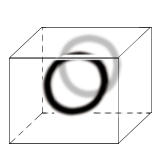
\includegraphics[width=4cm]{inudos/cubo1.png}
  	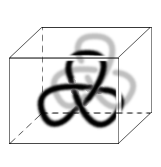
\includegraphics[width=4cm]{inudos/cubo2.png} 
  	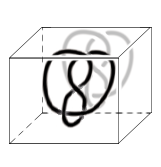
\includegraphics[width=4cm]{inudos/cubo3.png}
  	\centering
  	\caption{De izquierda a derecha: nudo trivial, nudo trébol, nudo de ocho.}
  	\label{trid} 
  \end{figure}

Nos interesa saber cuándo dos nudos son equivalentes: se puede pasar de uno a otro mediante deformaciones. Veámoslo formalmente:\\

Se dice que dos nudos son equivalentes si existe un homeomorfismo de  $\mathds{R}^{3}$ que nos lleve de un nudo al otro. \\


Podemos representar un nudo en el plano visualizando su proyección. Como hay muchas formas de representar un mismo nudo, podremos tener diferentes proyecciones que representen al mismo nudo. Se pueden ver dos proyecciones distintas de un mismo nudo en la figura \ref{cross1}. Algunos ejemplos básicos de proyecciones son los siguientes:\\
  \begin{figure}[h!]
  	
\includegraphics[width=3cm]{inudos/1.jpg}
  	
\includegraphics[width=3cm]{inudos/3f.png} 
  	
\includegraphics[width=3cm]{inudos/fig8.jpg}
  	\centering
  	\caption{Proyecciones del nudo trivial, nudo trébol, nudo de ocho.}
  	\label{uno} 
  \end{figure}
  
  Podemos ver en ellos una serie de cruces. En concreto en el nudo trébol tenemos 3 cruces y el nudo de ocho tenemos 4 cruces. El nudo trivial destaca porque puede tener proyecciones sin ningún cruce. No obstante, hay nudos con cruces que corresponden a proyecciones del nudo trivial. \\
  
    \underline{\textbf{Definición:}}\\
     Un \textbf{enlace} es una o más curvas cerradas disjuntas en $\mathds{R}^{3}$. Cada una de sus curvas recibe el nombre de componente.\\
     Por ejemplo, el siguiente enlace tiene dos componentes:
  \begin{figure}[h!]
  	
\includegraphics[width=2.7cm]{inudos/enlace.png}
  	\centering
  	\label{dos} 
  \end{figure}

    Por tanto, podemos ver un nudo como un caso particular de enlace en el que sólo tenemos una componente.\\
    
  Una de las cuestiones más interesantes en la teoría de nudos es la siguiente: \\
  ¿Dado un nudo, o alguna proyección suya, podremos saber si se trata del nudo trivial?. A lo largo de este proyecto trataremos de dar respuesta, en parte, a dicha cuestión.\\
  
%\bigskip
\section{Sobre su historia y aplicaciones.}
En el siglo XIX, ciertos físicos escoceses se preguntaban por la estructura de los átomos.\\
Estos científicos tomaron como base la teoría de Descartes, que afirmaba que el \textit{éter} era un fluido que ocupaba todo el espacio y transmitía la luz (éter lumínico), para desarrollar su modelo del átomo. \\
Aunque dichos físicos conocían la existencia de los elementos y que estaban formados por átomos, no conocían la propia estructura de los átomos. \\

Científicos como Peter Guthrie Tait y Willian Thomson llegaron a la teoría de que los átomos se concebían como vórtices, que podríamos ver como remolinos tubulares, en dicho fluido. Estos vórtices se encontraban anudados y en función del tipo de anudamiento darían lugar a un tipo de elemento u otro.\\
De este modo se plantearon que los diferentes nudos corresponderían a los diferentes elementos de la naturaleza. De acuerdo con la teoría, si conociésemos todos los nudos posibles, crearíamos la tabla de elementos que reemplazaría la tabla periódica actual. \\

Para hacernos una idea más clara, para Willian Thomson el nudo trébol podría corresponder con el átomo de helio, el nudo de ocho con el átomo de oxígeno....\\

Numerosos científicos contribuyeron a dicha teoría intentando crear la tabla de nudos pero a finales de este mismo siglo, Michelson-Morley demostró que el éter lumínico no existía y por tanto la teoría de los átomos de vórtice fue descartada. \\

Tras este hecho, la teoría de nudos perdió su interés hasta que fue objeto de estudio en Topología a principios del siglo XX.\\

Posteriormente esta rama de la topología de baja dimensión destacó por su gran interés en áreas como:
  \begin{enumerate}
  	\item Química: ya hemos visto que la teoría de nudos nace en este área.
  	\item Biología: se estudia la teoría de nudos en la estructura de ADN.\\
  	Conocemos como ácido desoxirribonucleico (ADN) a aquella molécula que se encuentra en el núcleo de nuestras células y, por tanto, que contiene nuestro código genético. Se trata de un elemento esencial para la vida. Es muy conocida su forma: se puede ver como dos cuerdas enrolladas formando un doble hélice. \\
  	
  	Su forma de doble hélice puede encontrarse cerrada por los extremos de forma que nos encontraríamos con la propia forma de un nudo. Las ideas que veremos en este proyecto, junto con algunas más, se pueden aplicar a estas estructuras de ADN.\\
  	
  	Además, esta estructura de ADN puede sufrir ciertas alteraciones producidas por la encima topoisomerasa. Lo interesante es que estas alteraciones se corresponden con algunos de los movimientos que veremos para los nudos.\\
  	
  	
  	\item Criptografía: 
  	La fuerte relación que veremos entre la teoría de nudos y la teoría de trenzas, hace que podamos establecer cierta relación entre la teoría de nudos y la criptografía. \\
  	
  	Haciendo uso de la criptografía tratamos de encontrar métodos para que el intercambio de información no sea comprensible por terceras personas.\\
  	
  	Algunos métodos para encriptar dicha información están inspirados en la teoría de trenzas. En concreto el problema de la conjugación de trenzas, que trata de estudiar la igualdad de dos trenzas haciendo uso de una tercera trenza, nos permitirá encriptar la información de forma segura. \\
  \end{enumerate}

%\section{Componiendo nudos.}\label{seccion3}
Supongamos que tenemos dos proyecciones J y K de nudos. Podemos definir un nuevo nudo a partir de ellos eliminando un arco de cada una de las proyecciones y conectando los 4 extremos finales de dos en dos mediante otros arcos de modo que no se añadan ni eliminen cruces.\\
A este nudo resultante le llamaremos \textbf{suma conexa} o composición de los dos nudos y se denotará como \textbf{J\#K}. A los nudos originales J y K les llamaremos \textbf{nudos factores}. \\

Por ejemplo, consideremos como nudos factores el nudo trébol y el nudo de ocho. 
\begin{figure}[h!]
	\subfigure[J]{
\includegraphics[width=2.5cm]{inudos/conexion1.jpg}} 
	\subfigure[K]{
\includegraphics[width=2.5cm]{inudos/fig8.jpg}}
	\centering
	\caption{Nudo trébol y nudo de ocho.}
	\label{comp1} 
\end{figure}

Haciendo la suma conexa de ambos nudos obtenemos el nudo composición:
\begin{figure}[h!]
	\subfigure[Haciendo la composición]{
\includegraphics[width=7cm]{inudos/conexion2.jpg} }
	\subfigure[J\#K]{
\includegraphics[width=7cm]{inudos/conexion3.jpg}}
	\centering
	\caption{Composición de nudo trébol y nudo de ocho.}
	\label{comp2} 
\end{figure}


El nudo trivial es un elemento identidad para la suma conexa: si hacemos la composición de un nudo cualquiera J con el nudo trivial, vamos a obtener el propio nudo J. Por ejemplo, seguimos considerando J como el nudo trébol y el nudo trivial como K. \\
\begin{figure}[h!]
	\centering
	\subfigure[J]{
\includegraphics[width=2.5cm]{inudos/conexion1.jpg} }
	\subfigure[K]{
\includegraphics[width=2.5cm]{inudos/1.jpg}}
	\caption{Nudo trébol y nudo trivial.}
	\label{comp3} 
\end{figure}

Su suma conexa nos seguiría dando el nudo factor J, es decir, el nudo trébol.\\

\begin{figure}[h!]
	\subfigure[Haciendo la composición]{
\includegraphics[width=8cm]{inudos/conexion4.jpg} }
	\subfigure[J\#K]{
\includegraphics[width=4cm]{inudos/conexion1.jpg}}
	\centering
	\caption{Composición de nudo trébol y nudo trivial.}
	\label{comp4} 
\end{figure}

\underline{\textbf{ Definición:}}\\
Diremos que un \textbf{nudo es primo} si no puede ser expresado como la suma conexa de dos nudos, a menos que uno de ellos sea el nudo trivial. \\

\underline{ \textbf{ Definición:}}\\
Diremos que un \textbf{nudo es compuesto} si no es el nudo trivial ni es un nudo primo.\\

Por ejemplo, los nudos trébol y nudo de ocho de la figura \ref{comp1} son nudos primos mientras que el nudo de la figura \ref{comp2} es un nudo compuesto. \\ 

Hay una gran variedad de nudos primos. Cualquier nudo puede ser expresado singularmente como suma conexa de nudos primos. En la tabla \ref{comp6} podemos ver los diferentes nudos primos que tienen menos de 8 cruces.\\
\begin{figure}[h!]
	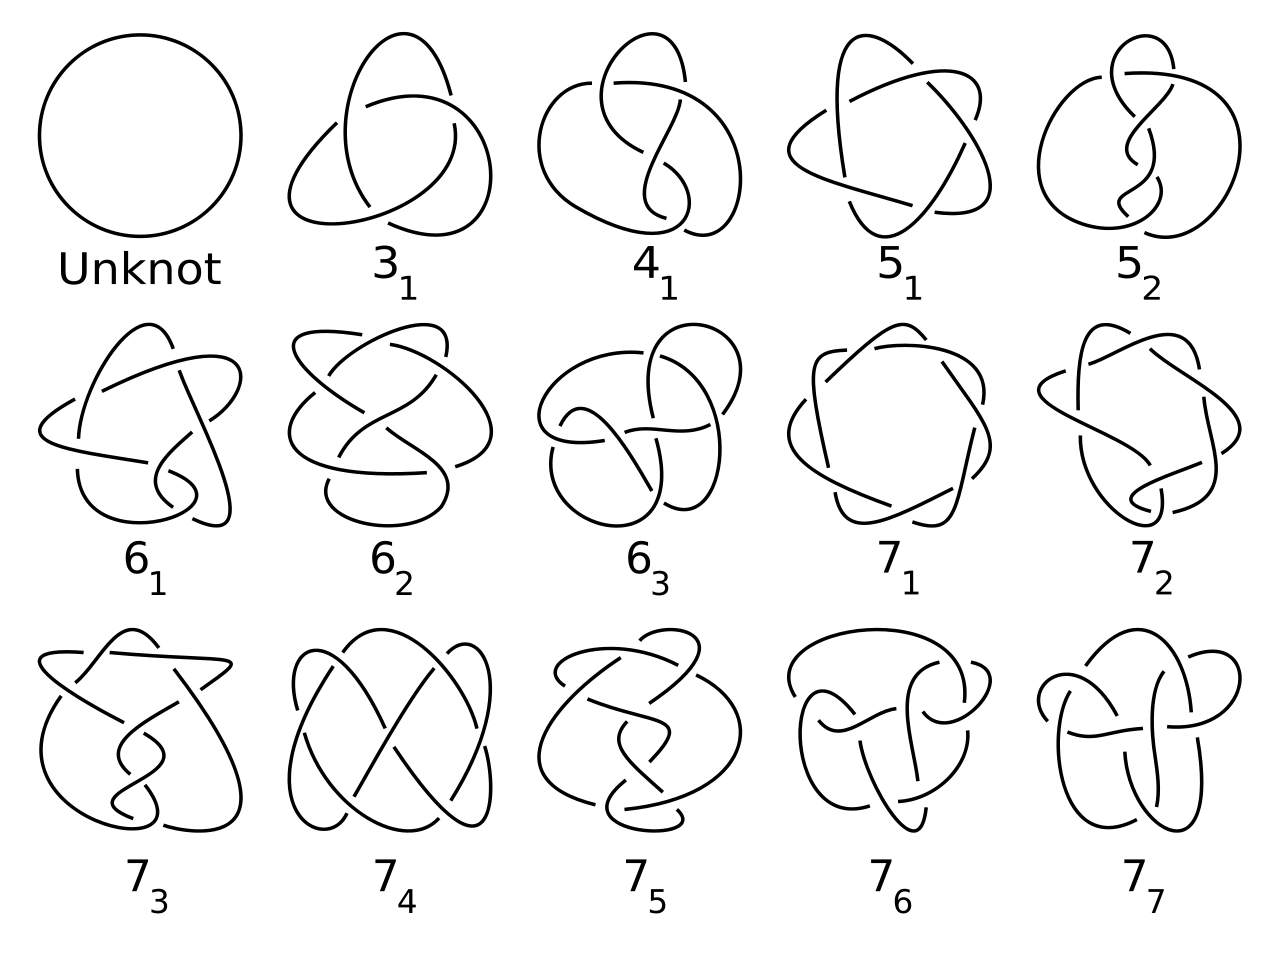
\includegraphics[width=14cm]{inudos/tableknot.png}
	\centering
	\caption{Composición de nudo trébol y nudo trivial.}
	\label{comp6} 
\end{figure}




Finalmente, es importante destacar el hecho de que la elección que hacemos de los arcos que eliminamos de cada uno de los nudos factores afecta al nudo composición. Por tanto, es posible construir dos nudos composición diferentes a partir del mismo par de nudos factores. Veamos esta idea con más detalle, para ello necesitamos:\\

\underline{\textbf{ Definición:}}\\
\textbf{ Un nudo orientado} es un nudo al que se le ha asignado una orientación, es decir, es un nudo que dispone de una dirección de viaje sobre él mismo. Esta orientación se indica mediante flechas en la proyección. \\

\underline{\textbf{ Definición:}}\\
\textbf{ Un nudo es invertible} si es equivalente a sí mismo con la orientación opuesta. \\

El problema de determinar si un nudo cualquiera es o no invertible no es para nada trivial.

Como ejemplo de nudo invertible nos podemos encontrar el nudo trébol, que vemos en la imagen \ref{comp5}.\\
\begin{figure}[h!]
	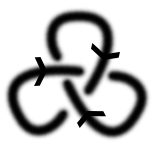
\includegraphics[width=3.5cm]{inudos/3fcon1.png}
	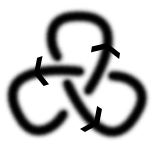
\includegraphics[width=3.5cm]{inudos/3fcon2.png}
	\centering
	\caption{Ambas orientaciones del nudo trébol.}
	\label{comp5} 
\end{figure}

Sean los dos nudos factores J y K a los que se asignamos una orientación. Tendremos dos formas posibles de hacer la composición: conectar con las orientaciones emparejadas o no emparejadas. \\
Todas las composiciones de los nudos cuyas orientaciones emparejan al componer, darán el mismo nudo composición. Todas las composiciones de los nudos cuyas orientaciones no emparejan al componer, también darán el mismo nudo composición. Sin embargo, es posible que la composición de los nudos cuyas orientaciones emparejen no de lugar al mismo nudo que haciendo la composición de los nudos cuyas orientaciones no emparejen. Serán el mismo si uno de los nudos factores es invertible.\\

Veamos un caso en el que la composición de dos mismos factores, genera nudos diferentes. Consideramos el nudo de la imagen \ref{comp7}.\\

\begin{figure}[h!]
	
\includegraphics[width=4cm]{inudos/817con.png}
	\centering
	\caption{Nudo factor J y K.}
	\label{comp7} 
\end{figure}
Si componemos el nudo consigo mismo conectando las orientaciones emparejadas y desemparejadas obtenemos nudos que no son equivalentes. Lo podemos comprobar visualmente en la Figura \ref{comp8}.

\begin{figure}[h!]
	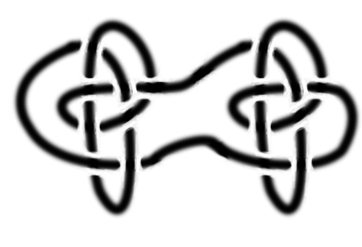
\includegraphics[width=7cm]{inudos/817def1.png}
	
\includegraphics[width=7cm]{inudos/817def2.png}
	\centering
	\caption{Las composiciones no son equivalentes.}
	\label{comp8} 
\end{figure}
%\bigskip
\section{Equivalencia de nudos: movimientos de Reidemeister.}\label{seccion4}
Dos nudos K1 y K2 serán equivalentes (K1 $\thicksim$ K2) si podemos distorsionar uno de ellos en el otro sin hacer ningún corte. \\

Para ver si dos proyecciones corresponden a nudos equivalentes, usaremos el concepto de isotopía plana. Más precisamente, definimos una \textbf{isotopía plana} de las proyecciones P1 y P2 de nudos como la aplicación continua $F: \mathds{R}^{2}$ x $[0,1] \rightarrow \mathds{R}^{2}$ tal que $F_{0}=identidad$, $F_{1}(P1) = P2$ y $F_{t}$ es un homeomorfismo $\forall t$.\\

Los movimientos de Reidemeister que vamos a ver a continuación nos permiten cambiar la proyección de un nudo de modo que se cambie la relación entre los cruces pero que no cambie el nudo al que representa la proyección. \\
Cada uno de estos movimientos es una isotopía:\\

\textbf{Primer movimiento de Reidemeister - R1}\\
En cualquier zona de la proyección nos permite añadir o eliminar un giro tal y como vemos en la figura \ref{movi1}.
  \begin{figure}[h!]
  	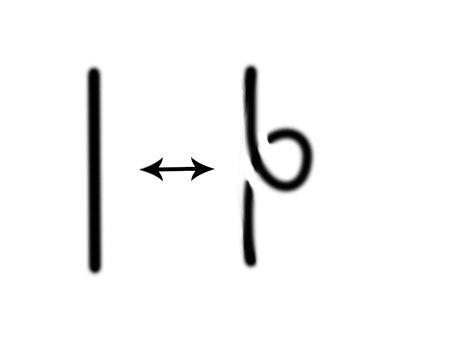
\includegraphics[width=5cm]{inudos/movi1.png}
  	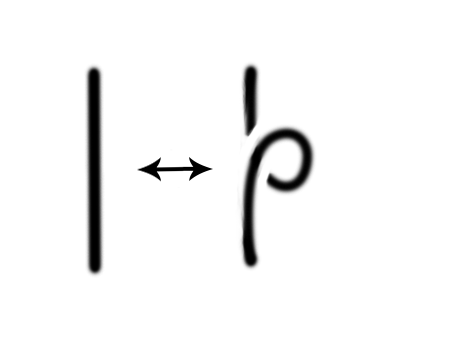
\includegraphics[width=5cm]{inudos/movi2.png}
  	\centering
  	\caption{Primer movimiento Reidemeister.}
  	\label{movi1} 
  \end{figure}
  
	\textbf{Segundo movimiento de Reidemeister - R2.}\\
Nos permite añadir o eliminar dos cruces del nudo como se ve en la figura \ref{movi2}.
    \begin{figure}[h!]
    	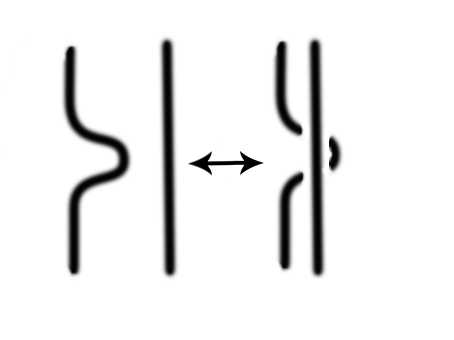
\includegraphics[width=7cm]{inudos/movi3.png}
    	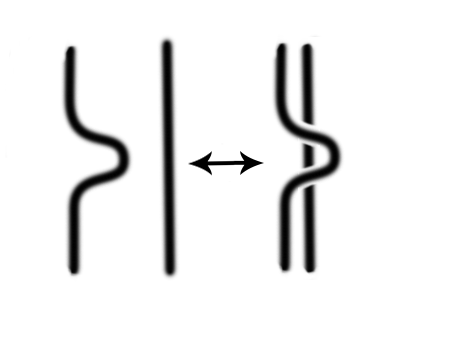
\includegraphics[width=7cm]{inudos/movi4.png}
    	\centering
    	\caption{Segundo movimiento de Reidemeister.}
    	\label{movi2} 
    \end{figure}
    
	\textbf{Tercer movimiento de Reidemeister - R3.}\\
Nos permite deslizar una hebra del nudo de un lado de un cruce al otro lado del cruce. Veamos la figura \ref{movi3} para aclarar la idea.
      \begin{figure}[h!]
      	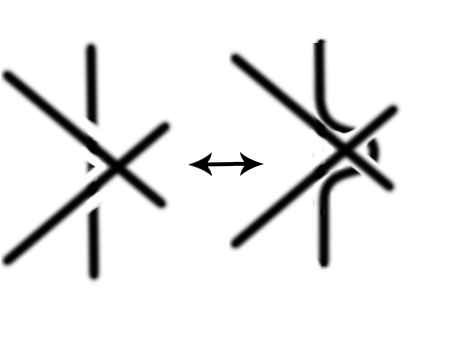
\includegraphics[width=7cm]{inudos/movi5.png}
      	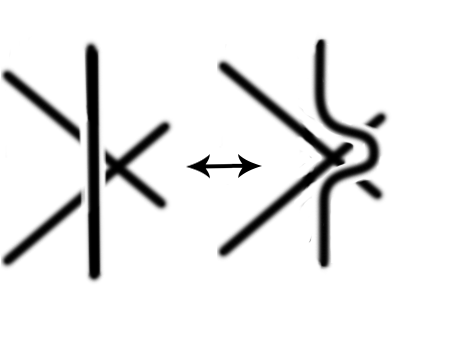
\includegraphics[width=7cm]{inudos/movi6.png}
      	\centering
      	\caption{Tercer movimiento de Reidemeister.}
      	\label{movi3} 
      \end{figure}
  

\begin{teo} \textbf{Teorema de Reidemeister \cite{5}.} Sean P1 y P2 las proyecciones que representan a dos nudos K1 y K2, respectivamente. Entonces, K1 $\thicksim$ K2 si, y solo si, P1 y P2 están conectados por una secuencia finita de movimientos de Reidemeister e isotopías planas.
\end{teo}

Veamos un ejemplo en el que vemos la equivalencia de dos proyecciones, que en un primer momento podrían no parecernos equivalentes:
  \begin{figure}[h!]
  	\subfigure[P1]{
\includegraphics[width=3cm]{inudos/3f.png}}
  	\subfigure[R1]{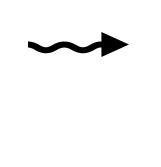
\includegraphics[width=2cm]{inudos/flecha.png}}
  	
\includegraphics[width=3cm]{inudos/3fseg.png}
  	\subfigure[R3]{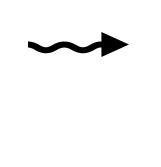
\includegraphics[width=2cm]{inudos/flecha.png}}
  	
\includegraphics[width=3cm]{inudos/fase3.png}
  	\subfigure[Isotopia]{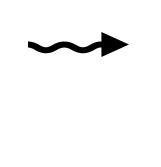
\includegraphics[width=2cm]{inudos/flecha.png}}
  	
\includegraphics[width=3cm]{inudos/fase4.png}
  	\subfigure[R3]{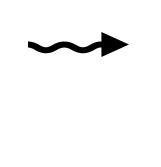
\includegraphics[width=2cm]{inudos/flecha.png}}
  	
\includegraphics[width=3cm]{inudos/fase5.png}
  	\subfigure[R1]{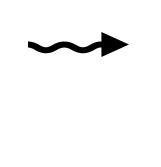
\includegraphics[width=2cm]{inudos/flecha.png}}
  	
\includegraphics[width=3cm]{inudos/fase6.png}
  	\subfigure[Isotopia]{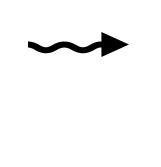
\includegraphics[width=2cm]{inudos/flecha.png}}
  	
\includegraphics[width=3cm]{inudos/fase7.png}
  	\subfigure[Isotopia]{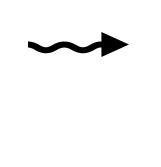
\includegraphics[width=2cm]{inudos/flecha.png}}
  	\subfigure[P2]{
\includegraphics[width=3cm]{inudos/fase8.png}}
  	\centering
  	\caption{Equivalencia de dos proyecciones de nudos.}
  	\label{algosj} 
  \end{figure}

Gracias a dicho teorema podremos estudiar si dos proyecciones representan el mismo nudo. Para ello tendremos que encontrar una secuencia de movimientos de Reidemeister que nos lleve de una proyección a la otra. Sin embargo, este proceso puede no tener el número de movimientos intermedios limitado por lo que no tiene mucho sentido implementarlo.\\
 
 Aunque este teorema no nos permita ver de una forma cómoda la equivalencia entre dos nudos en la práctica (por la fuerte complejidad) si que nos permite obtener una conclusión esencial:\\
 
 Si una propiedad de un nudo no cambia al aplicarle cualquiera de estos tres movimientos de Reidemeister, entonces esta propiedad no va a cambiar por muchas deformaciones que se le hagan al nudo. En definitiva, si un nudo cumple cierta propiedad y otro nudo no la cumple, esos nudos no podrán ser equivalentes. Incidiremos en esta idea en la siguiente Sección \ref{seccion5}.
 
%\section{Algunos invariantes.}\label{seccion5}
Suponga que cierto día ha ido a trabajar con su portátil fuera de casa y se lo ha dejado olvidado. Cuando te das cuenta, vuelves a buscarlo pero ya no está. Pasan unos días y un amigo te comenta que se ha encontrado un portátil con $x$ número de puertos, procesador $y$ y modelo $z$.\\

Es claro que si alguna de esas características no fuese la de tu portátil, tendrías claro que no es el tuyo. Pero resulta que tu portátil tiene exactamente las mismas características. Piensas que tal vez sea tu portátil pero no tienes garantía de que realmente lo sea. \\

Algo similar, aplicado a nudos, es lo que vamos a tratar de ver en esta sección. ¿Dadas dos proyecciones, podremos decir que representan al mismo nudo? Vamos a tratar de estudiar ciertos invariantes sobre los nudos. Al igual que ocurría con el caso del portátil, si dos proyecciones tienen valores de un invariante distintos podremos decir que no representan al mismo nudo. Sin embargo, si ambos tienen valores de un invariante iguales no podremos saber si se trata del mismo nudo. Tendremos que estudiar otros invariantes de nudos. \\

¿Y si estudiamos una gran cantidad de invariantes de dos proyecciones y siempre toman los mismos valores?¿Podremos garantizar que son equivalentes? La respuesta es clara, no. Tendremos que analizar en mayor detalle las proyecciones, pero puede ser que no lleguemos a obtener un conclusión definitiva. \\


Por tanto, el estudio de invariantes de los nudos nos va a permitir saber si dos nudos pueden ser (destacamos, que no quiere decir que lo sean) o no son equivalentes.\\


Antes de ver algunos de los invariantes de nudos más conocidos y útiles vamos a dar una definición formal de lo que se conoce como un invariante:\\

\underline{\textbf{Definición:}} \\
Un \textbf{invariante} de un nudo (o de un enlace) es una propiedad que no cambia cuando el nudo sufre deformaciones en el espacio. \\



\begin{center}
	\subsection{Número de componentes:}
\end{center}
Es uno de los invariantes de enlaces más sencillos que nos podemos encontrar y que ya hemos comentado ligeramente en las secciones anteriores.\\

Cada componente de un enlace es una curva disjunta del mismo. En la Figura \ref{inv1} vemos un enlace con dos componentes. 
\begin{figure}[h!]
	
\includegraphics[width=2.7cm]{inudos/enlace.png}
	\centering
	\caption{Enlace con dos componentes.}
	\label{inv1} 
\end{figure}

Al aplicarle a un enlace cualquier transformación no se le puede añadir ni eliminar ninguna componente. De modo que este invariante no nos va a permitir comparar nudos, pues todo nudo tiene una sola componente. \\

\bigskip
\begin{center}
	\subsection{Crossing number:}
\end{center}
Sea un nudo K. Su \textbf{crossing number} es el menor número de cruces que se encuentra en cualquier proyección del nudo. Se denota como $c(K)$. \\

Esto nos lleva a deducir el nudo K tendrá como mínimo c(K) cruces por muchas transformaciones que se haga a sus proyecciones.\\

Aunque es un invariante sencillo de visualizar, no es fácil de obtener: puede ser que al estudiar muchas proyecciones de un nudo pensemos que su número de cruces es $n$, sin embargo pueden existir otras proyecciones del nudo que no conocemos con menor número de cruces. Por este motivo, no vamos a trabajar posteriormente con este invariante.\\

Para dejarlo más claro vamos a ver un ejemplo.\\
Consideramos la proyección de la primera figura \ref{cross1}. Podemos pensar que el número de cruces del nudo sería 4 (ver los 4 cruces de la figura a). Sin embargo, esta proyección es equivalente a la proyección que vamos en la figura b, que tiene como número de cruces el valor 3. Por tanto, el número de cruces del nudo, que es el nudo trébol, es 3. 
\begin{figure}[h!]
	\centering
	\subfigure[4 cruces]{
\includegraphics[width=3.4cm]{inudos/3fseg.png}}
	\subfigure[3 cruces]{
\includegraphics[width=3.4cm]{inudos/3f.png}}
	\caption{Crossing number del nudo trébol.}
	\label{cross1} 
\end{figure}  


\begin{center}
	\subsection{Tricolorabilidad:}
\end{center}
Para definir este invariante de enlaces, tenemos que conocer unos conceptos previos:\\
Entendemos por undercrossing y overcrossing a un recorrido en el cruce de la proyección de un nudo que nos lleva por encima o por debajo en el cruce. \\

Veamos la imagen \ref{tric1} donde queda representado:\\
\begin{figure}[h!]
	\centering
	
\includegraphics[width=7cm]{inudos/cruce.png}
	\caption{Tipo de cruce.}
	\label{tric1} 
\end{figure}

\underline{\textbf{Definición:}}\\
Una\textbf{ hebra }de una proyección de un enlace es una región de cuerda del enlace que va desde un undercrossing a otro undercrossing atravesando sólo overcrossings.\\ 

\underline{\textbf{Definición:}}\\
Una proyección de un enlace es tricolorable si cada una de las hebras de la proyección puede ser coloreada con uno de tres colores diferentes de modo que en cada cruce o los 3 colores se junten o se junte un sólo color. En este caso diremos que el enlace es \textbf{tricolorable}. 

\begin{teo}
	La tricolorabilidad se perserva mediante movimientos de Reidemeister.
	\begin{proof}
		Supongamos que partimos de una proyección de un nudo que es tricolorable y vamos a aplicarle los movimientos de Reidemeister. Tendremos que ver que la proyección final es tricolorable. Podemos centrarnos en la zona de la proyección a la que se le aplica el movimiento. Veamos qué ocurre al aplicar cada movimiento:\\
		
		\underline{R1:}
		En este caso sólo se puede dar que tengamos un sólo color. Al aplicar el movimiento R1 seguiremos utilizando ese mismo color, de modo que la proyección modificada seguirá siendo tricolorable. 
		\begin{figure}[h!]
			\centering
			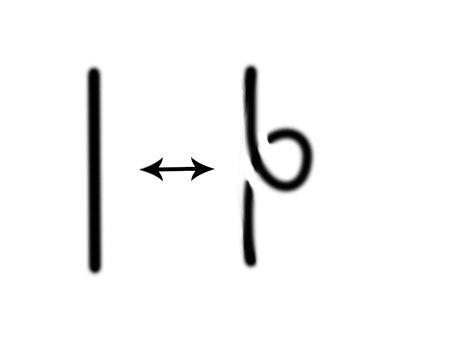
\includegraphics[width=5.5cm]{inudos/movi1.png}
			\includegraphics[width=5.5cm]{inudos/movi2.png}
			\caption{}
			\label{demotri1} 
		\end{figure}
		
		\underline{R2:}
		Supongamos que el coloreado inicial se ha realizado con un sólo color. Al igual que con el movimiento R1, no tendríamos ninguna dificultad pues al aplicar el movimiento R2 seguiremos coloreando con el mismo color y la proyección seguirá siguiendo tricolorable. \\
		\begin{figure}[h!]
			\centering
			\includegraphics[width=5.5cm]{inudos/movi3.png}
			\includegraphics[width=5.5cm]{inudos/movi4.png}
			\caption{}
			\label{demotri2} 
		\end{figure}
		
		Ahora tenemos otra segunda opción de coloreado en la proyección inicial y es que en ambos cruces posibles usemos los 3 colores posibles. Se puede ver en la figura \ref{demotri3}. Se observa que la proyección sigue siendo tricolorable. 
		\begin{figure}[h!]
			\centering
			\includegraphics[width=8.3cm]{inudos/movi3tri.png}
			\includegraphics[width=8.3cm]{inudos/movi4tri.png}
			\caption{}
			\label{demotri3} 
		\end{figure}
		
		\underline{R3:}
		Este movimiento tiene más complejidad pues tenemos 3 cruces posibles. Analizamos todos los casos posibles y vemos que nos podemos reducir a cinco situaciones. Veamos en la figura \ref{demotri4} cómo sería el cambio de color en cada caso para confirmar que las proyecciones resultantes al aplicar el movimiento siguen siendo tricolorables.
		\begin{figure}[h!]
			\centering
			\includegraphics[width=8cm]{inudos/movi5.png}
			\includegraphics[width=8cm]{inudos/movi5tri1.png}
			\includegraphics[width=8cm]{inudos/movi5tri2.png}
			\includegraphics[width=8cm]{inudos/movi5tri3.png}
			\includegraphics[width=8cm]{inudos/movi5tri4.png}
			\caption{}
			\label{demotri4} 
		\end{figure}
		
		Concluimos que si tenemos una proyección tricolorable y aplicamos los movimientos de Reidemeister, la proyección resultante sigue siendo tricolorable. \\
		Si la proyección de partida no fuese tricolorable, la proyección resultante tampoco podría ser tricolorable: supongamos que la proyección resultante es tricolorable, por el razonamiento que hemos seguido anteriormente, tendríamos que tener que la proyección inicial sería tricolorable llegando a contradicción. 
		
	\end{proof}
\end{teo}


Haciendo uso de este invariante podemos demostrar que el nudo trivial y el nudo trébol no son equivalentes, es decir, son topológicamente distintos. Esto se debe a que el nudo trébol es tricolorable pero el nudo trivial no lo es. Podemos verlo en la imagen \ref{Tric2}.\\
\begin{figure}[h!]
	\centering
	\subfigure[No tricolorable]{\includegraphics[width=4cm]{inudos/1.jpg}}
	\subfigure[Tricolorable]{\includegraphics[width=4cm]{inudos/3ftri.png}}
	\caption{Dos nudos no equivalentes.}
	\label{Tric2} 
\end{figure} 


Este hecho confirma que existe al menos un nudo distinto del nudo trivial. Es más, todo nudo que sea tricolorable será distinto del nudo trivial.\\

Sin embargo, este invariante no es muy potente en el sentido de que sólo clasifica los enlaces en tricolorables y no tricolorables y sólo podremos afirmar que dos proyecciones representan a diferentes nudos si una de ellas es tricolorable y la otra no lo es.   


\bigskip
\begin{center}
	\subsection{Unknotting number:}\label{subunk}
\end{center}
Supongamos que tenemos la proyección de un nudo no trivial. Modificar la proyección para que un undercrossing pase a ser un overcrossing, o viceversa, no es un movimiento válido pues estamos intersecando la cuerda. Sin embargo, es un movimiento interesante ya que nos llevará al nudo trivial. \\

\underline{\textbf{Definición:}}
Se define el \textbf{número de desanudamiento} de un nudo como el menor número de cambios en los cruces necesarios para desanudarlo, es decir, para llegar al nudo trivial. Se denota como $u(K)$. \\

Es claro que en un número finito de pasos conseguiremos obtenemos el número de desanudamiento: Recorremos el nudo con cierta orientación y al llegar a un cruce, si no hemos pasado anteriormente por él y es un undercrossing, lo convertimos en overcrossing. \\ 

Podemos ver, en la figura \ref{unk1}, que el número uno es el número de desanudamiento para el nudo trébol. El punto de partida lo indicamos con un punto grueso.
\begin{figure}[h!]
	\centering
	\subfigure[Nudo de partida]{\includegraphics[width=3.4cm]{inudos/3fcon1start.png}}
	\subfigure[Nudo modificado]{\includegraphics[width=3.4cm]{inudos/3fcon1negstart.png}}
	\caption{Unknotting number trébol.}
	\label{unk1} 
\end{figure}

\bigskip
\begin{center}
	\item \subsection{Polinomio de Alexander:}\label{alenudos}
\end{center}
Anteriormente hemos visto algunos invariantes geométricos y numéricos que nos pueden ayudar en la tarea de comprobar si dos proyecciones representan al mismo nudo. Ahora vamos a ver un invariante polinómico que estudiaremos con más detalle pues será uno de los puntos fuertes que implementaremos para resolver, en parte, la cuestión. \\

Se trata de un polinomio, con variable $t$, para nudos orientados. En 1969, se probó que dicho polinomio puede calcularse computacionalmente haciendo uso de dos reglas:
\begin{itemize}
	\item \underline{Regla 1:} \\
	El polinomio de Alexander del nudo trivial es el polinimio trivial equivalente a 1. Esta regla se representa como $\vartriangle$($\bigcirc$)= 1
\end{itemize}

Para poder exponer la segunda regla tenemos que conocer antes las siguientes ideas. \\
Consideramos el enlace orientado de partida. Si nos centramos en uno de sus cruces, podemos crear tres nuevos enlaces orientados exactamente iguales al de partida variando únicamente en este cruce seleccionado. A cada uno de estos nuevos enlaces le establecemos uno de estos nuevos cruces:
\begin{enumerate}
	\item $L_{+}$: El cruce seleccionado se establece como positivo.
	\item $L_{-}$: El cruce seleccionado se establece como negativo.
	\item $L_{0}$: El cruce seleccionado se elimina.
\end{enumerate}
Podemos ver estos nuevos cruces en la figura \ref{alex1}.\\

\begin{figure}[h!]
	\centering
	\subfigure[$ L_{+} $]{\includegraphics[width=4cm]{inudos/pro1.png}}
	\subfigure[$ L_{-} $]{\includegraphics[width=4cm]{inudos/pro2.png}}
	\subfigure[$ L_{0} $]{\includegraphics[width=4cm]{inudos/pro3.png}}
	\caption{Tipos de cruces.}
	\label{alex1} 
\end{figure}


\begin{itemize}
	\item \underline{Regla 2:} \\
	Esta regla se representa como $\vartriangle(L_{+}) - \vartriangle(L_{-}) +  (t^{\frac{1}{2}} - t^{\frac{-1}{2}}) \vartriangle(L_{0})  = 0$
\end{itemize}

Veamos cómo se calcularía el polinomio de Alexander con el nudo trébol:\\
Como el nudo de partida tiene más de un cruce, tenemos que aplicarle la segunda regla. Consideraremos como cruce a cambiar el que nos encontramos más a la izquierda aunque podríamos considerar cualquier otro cruce. Generamos los tres nuevos enlaces haciendo el cambio en el cruce. Sus proyección se pueden ver en la figura \ref{alex2}. Las llamamos A, B y C por comodidad. 
\begin{figure}[h!]
	\centering
	\subfigure[A]{\includegraphics[width=5cm]{inudos/3fcon1.png}}
	\subfigure[B]{\includegraphics[width=5cm]{inudos/3fcon1neg.png}}
	\subfigure[C]{\includegraphics[width=5cm]{inudos/doble1b.png}}
	\caption{}
	\label{alex2} 
\end{figure}

Al aplicar la segunda regla tendremos:\\
\begin{equation}
\vartriangle(A) - \vartriangle(B) +  (t^{\frac{1}{2}} - t^{\frac{-1}{2}}) \vartriangle(C)  = 0.
\end{equation}
Sabemos que $\vartriangle(B)$ = $\vartriangle$($\bigcirc$)= 1. Luego nos quedaría la ecuación:
\begin{equation}
\vartriangle(A) +  (t^{\frac{1}{2}} - t^{\frac{-1}{2}}) \vartriangle(C)  = 1.
\end{equation}
Ahora necesitamos conocer el valor de $\vartriangle(C)$. Al igual que ocurría anteriormente, la proyección de este nuevo nudo tiene más de un cruce de modo que vamos a aplicarle la segunda regla. Esta vez seleccionamos el cruce superior como cruce que se modifica en los nuevos nudos. Obtenemos las proyecciones que vemos en la figura \ref{alex3}, a las que llamaremos D y E. 
\begin{figure}[h!]
	\centering
	\subfigure[D]{\includegraphics[width=5cm]{inudos/doble2b.png}}
	\subfigure[E]{\includegraphics[width=5cm]{inudos/doble3b.png}}
	\caption{}
	\label{alex3} 
\end{figure}

Al aplicar la segunda regla tendremos:\\
\begin{equation}
\vartriangle(C) - \vartriangle(D) +  (t^{\frac{1}{2}} - t^{\frac{-1}{2}}) \vartriangle(E)  = 0.
\end{equation}

Sabemos que $\vartriangle(E)$ = $\vartriangle$($\bigcirc$)= 1. Además $\vartriangle(D)$ = $\vartriangle$($\bigcirc$ $\bigcirc$)= 0. Luego nos quedaría la ecuación:
\begin{equation}
\vartriangle(C) = -  (t^{\frac{1}{2}} - t^{\frac{-1}{2}}).
\end{equation}

Volviendo a la ecuación (2) tendemos:
\begin{equation}
\vartriangle(A) =  (t^{\frac{1}{2}} - t^{\frac{-1}{2}})^{2} + 1 = t^{-1} -1 + t.
\end{equation}
Luego $ t^{-1} -1 + t $ es el polinomio de Alexander del nudo trébol. \\

\bigskip
Es importante destacar el hecho de que podemos tener un nudo no trivial que tenga como polinomio de Alexander el polinomio trivial equivalente a 1. Por este motivo, con dicho invariante no podemos distinguir cualquier nudo del nudo trivial. \\

¿Mediante estas dos reglas podremos obtener siempre el polinomio de Alexander en tiempo finito? La respuesta es afirmativa, veámoslo:\\

La idea que vamos a seguir en este proceso será reducir las proyecciones, a las que le queremos obtener el polinomio de Alexander, hasta llegar al nudo trivial. Reducir estas proyecciones quiere decir ir modificando sus cruces obteniendo $L_{+}$, $L_{-}$ y $L_{0}$ . Como veíamos en el invariante de la sección \ref{subunk}, a cualquier proyección le podemos aplicar una secuencia finita de cambios en los cruces de modo que resulte el nudo trivial. Por tanto, este procedimiento tendrá fin en una secuencia finita de pasos.\\

Al ir considerando los distintos nudos de la proyección, obtendremos dos nuevas proyecciones en cada paso. Con estas nuevas proyecciones podremos formar lo que se denomina \textbf{ árbol de resolución}. En la figura \ref{alex4} podemos ver el árbol de resolución del nudo trébol.\\

\begin{figure}[h!]
	\centering
	\includegraphics[width=18cm]{inudos/arbol.png}
	\caption{Árbol de resolución del nudo trébol.}
	\label{alex4} 
\end{figure}

\underline{\textbf{Definición:}}\\
Se define la \textbf{profundidad de un nudo} (o enlace) como el mínimo número de niveles que nos encontramos en los árboles de resolución del nudo. \\

Esta profundidad del nudo es un invariante que además nos permite medir la complejidad que supondrá el cálculo del polinomio de Alexander. \\

El árbol de resolución del nudo trébol que vemos en la figura \ref{alex4} tiene una profundidad de 2 niveles (la proyección inicial no se cuenta como nivel). Es importante destacar que el único nudo que tiene profundidad de nudo igual a 0 es el nudo trivial. \\
%\bigskip
\section{Notación de nudos.}
Ya sabemos qué son los nudos y algunas nociones esenciales sobre los mismos, pero aún no sabemos asociar una notación concreta a un nudo. En esta sección vamos a ver algunas de las notaciones más comunes de los nudos. 

\begin{center}
	\item \subsection{Notación de Dowker:}
\end{center}
Se trata de una notación muy sencilla para describir la proyección de un nudo. La notación en sí es una secuencia de números enteros, veamos cómo se obtiene:\\

Consideramos una orientación en la proyección de n cruces y asignamos el valor 1 al primer cruce que nos encontremos. Continuamos por la proyección y asignamos el valor 2 al siguiente cruce. Vamos repitiendo el proceso hasta pasar por cada cruce un par de veces (una vez por el undercrossing y otra por el overcrossing). Como resultado tendremos un número par y un número impar por cada cruce de la proyección. \\

Finalmente es necesario asignar los signos a cada uno de estos $2n$ números. Los números pares que correspondan a un overcrossing tendrán signo negativo. Veamos un ejemplo con el nudo trébol que podemos ver en la figura \ref{dow1}:\\
   \begin{figure}[h!]
   	\centering
   	\includegraphics[width=4cm]{inudos/3fcon2dow.png}
   	\caption{Numeración de cruces-Dowker.}
   	\label{dow1} 
   \end{figure}
   
  Tendríamos los pares (1,-4), (3,-6) y (5,2). La notación de Dowker sería -4 -6 2 pues nos quedamos únicamente con los números pares en el orden que indican los números impares.\\

\begin{center}
	\item \subsection{Notación de Gauss:}
\end{center}
La notación de Gauss es una notación parecida a la de Dowker. Consideremos de nuevo una orientación en la proyección de n cruces de un nudo.\\

En este caso cada vez que pasamos por un cruce, tendremos un solo número asignado. De este modo la secuencia de números de la notación se compone de $2n$ elementos con valores desde 1 hasta n, cada uno de ellos repetido dos veces.\\

Consideramos una orientación en la proyección de n cruces y asignamos el valor 1 al primer cruce que nos encontremos. Realizamos el siguiente proceso: continuamos por la proyección hasta el siguiente cruce. Si ya hemos pasado por él, anotamos el número de cruce que tenga asociado. Si no hemos pasado anteriormente por él, asignamos el siguiente número de cruce.\\

Finalmente es necesario asignar los signos a cada uno de esos $2n$ números. Los números que representen uncrossings tendrán signo negativo. Veamos la notación de Gauss para el nudo trébol.\\
   \begin{figure}[h!]
   	\centering
   	\includegraphics[width=4cm]{inudos/3fcon2gaus.png}
   	\caption{Numeración de cruces-Gauss.}
   	\label{gaus1} 
   \end{figure} 
Si vamos haciendo el recorrido partiendo desde el punto grueso indicado tendríamos la secuencia de números: -1 2 -3 1 -2 3. Esta sería su notación de Gauss.

\begin{center}
	\item \subsection{Notación de Conway:}
\end{center}
Por último vamos a ver una notación que puede resultar algo más compleja pero que tiene gran uso e interés, sobre todo en la teoría del ADN. \\

\underline{\textbf{Definición:}}\\
Un \textbf{enredo} o tangle de una proyección de un enlace es una región de la proyección rodeada por una bola de modo que las dos cuerdas enlazadas de la proyección tocan la bola exactamente en cuatro puntos. A estos puntos los denotaremos como NO, NE, SO y SE.\\

En la figura \ref{conw1} vemos un enredo general y un ejemplo particular de un enredo.\\
   \begin{figure}[h!]
   	\centering
   	\subfigure[Enredo general]{\includegraphics[width=4.5cm]{inudos/en1.png}}
   	\subfigure[Ejemplo de enredo]{\includegraphics[width=4.5cm]{inudos/en2.png}}
   	\caption{Enredos}
   	\label{conw1} 
   \end{figure} 

Pero la idea es trabajar con enredos más sencillos como son los que vemos en la figura \ref{conw2}. La notación se corresponde con el número de cruces que tiene el enredo con signo positivo y negativo según se ve en las imágenes.\\
   \begin{figure}[h!]
   	\centering
   	\subfigure[Enredo $\infty$]{\includegraphics[width=3cm]{inudos/en3.png}}
   	\subfigure[Enredo 0]{\includegraphics[width=3cm]{inudos/3enrot.png}}
   	
   	\subfigure[Enredo 4]{\includegraphics[width=8cm]{inudos/en4.png}}
   	
   	\subfigure[Enredo -4]{\includegraphics[width=8cm]{inudos/en4conneg.png}}
   	\caption{Tipos básicos de enredos.}
   	\label{conw2} 
   \end{figure} 

Haciendo uso de estos enredos básicos podemos construir nuevos enredos uniendo, respectivamente, los extremos NE y SE de un enredo con los extremos NO y SO del otro enredo. A esta operación se le conoce como suma de enredos.\\
Además, disponemos de una operación de multiplicación: reflejaremos el primer enredo y hacemos la operación de suma.\\
A los enredos construidos con estas operaciones se les conoce con \textbf{enredos racionales}. Podemos ver un esquema básico estas dos operaciones en la imagen \ref{conw3}:\\
   \begin{figure}[h!]
   	\centering
   	\subfigure[Operacion suma]{\includegraphics[width=8cm]{inudos/ensum.png}}
   	\subfigure[Operacion multiplicacion]{\includegraphics[width=8cm]{inudos/enmul.png}}
   	\caption{Operaciones con enredos.}
   	\label{conw3} 
   \end{figure}

En la figura \ref{conw4} podemos ver un ejemplo de un enlace más complejo:
\begin{figure}[h!]
	\centering
	\includegraphics[width=4cm]{inudos/en5fin.png}
	\caption{Enlace -2 3 2}
	\label{conw4} 
\end{figure}

A partir de estos enredos podemos construir proyecciones de nudos enlazando los puntos NO con NE y los puntos SO con SE. La notación del nudo corresponde con la notación que le damos a su enredo.\\ 

Nos interesa ver si dos proyecciones de nudos representan al mismo nudo, luego nos interesa ver si dos enredos son equivalentes. Veamos qué quiere decir que sean equivalentes:\\

\underline{\textbf{Definición:}}\\
Diremos que dos enredos son equivalentes si podemos pasar de un enredo al otro mediante los movimientos de Reidemeister, que vimos en la sección \ref{seccion4}, manteniendo los cuatro extremos fijos en la bola imaginaria. \\

Ver si dos enredos son equivalentes por definición no es viable de modo que vamos a aplicar otro método: consiste en calcular la fracción continua asociada a cada enredo.\\

\underline{\textbf{Definición:}}\\
Sea un enredo con notación $a_{n}...a_{1}a_{0}$. Su\textbf{ fracción continua} es una expresión del tipo:
\begin{equation}
    a_{0} + \frac{1}{a_{1} + \frac{1}{a_{2} + \frac{1}{...a_{n}}}}
\end{equation}
siendo $a_{i} \in \mathds{Z},  \forall i = 0,1,..,n.$\\

\begin{teo}
Dos enredos racionales son equivalentes si y solo si sus fracciones continuas toman el mismo valor. 
\end{teo}

Veamos un ejemplo. Consideramos los enredos racionales -2 3 2 y 3 -2 3 que vemos en la figura \ref{conw5}.\\
\begin{figure}[h!]
	\centering
	\subfigure[Enlace -2 3 2]{\includegraphics[width=4cm]{inudos/en5fin.png}}
	\space
	\subfigure[Enlace 3 -2 3]{\includegraphics[width=4cm]{inudos/en6fin.png}}
	\caption{Enlaces equivalentes}
	\label{conw5} 
\end{figure}

A simple vista resulta difícil confirmar que sean equivalentes. Vamos a obtener sus fracciones continuas asociadas:\\
$-2 \hspace{1cm} 3 \hspace{1cm} 2 \hspace{1cm}$ tiene fracción continua
\begin{equation}
 2 + \frac{1}{3 + \frac{1}{-2}} = \frac{12}{5}
\end{equation}

$3 \hspace{1cm} -2 \hspace{1cm} 3 \hspace{1cm}$ tiene fracción continua
\begin{equation}
3 + \frac{1}{-2 + \frac{1}{3}} = \frac{12}{5}
\end{equation}
Ambas fracciones continuas son iguales, luego los enredos -2 3 2 y 3 -2 3 son equivalentes. 

%\section{Conexión con distintas teorías.}\label{seccion7}
\begin{center}
	\item \subsection{Teoría de grafos:}
\end{center}

\underline{\textbf{Definición:}}\\
Un \textbf{grafo} es un par $ (V,A) $ de conjuntos, junto con la aplicación 
\begin{center}
	 $  \gamma :A \rightarrow$ \{\{$u,v$\} / $u,v \in V$\}  
\end{center}
Al conjunto de puntos V se se llama conjunto de vértices y al conjunto A le llamaremos conjunto de aristas. \\

\underline{\textbf{Definición:}}\\
Un \textbf{grafo plano} $ G $ es un grafo que permanece en el plano.\\

Podemos ver varios ejemplos en la figura \ref{graf1}.\\
\begin{figure}[h!]
	\centering
	\includegraphics[width=3.5cm]{inudos/grafo.png}
	\includegraphics[width=4cm]{inudos/pgrafo.png}
	\caption{Ejemplos de grafos planos.}
	\label{graf1} 
\end{figure}

A partir de la proyección de un nudo (o de un enlace en general) podemos generar su grafo plano asociado. Para ello tendremos que realizar el siguiente proceso:\\

Sombreamos las regiones de la proyección que estén de modo que la región externa al nudo se quede sin sombrear y situamos un vértice en cada zona. Unimos los vértices con aristas que pasan por los cruces de la proyección. Ya tendríamos el grafo plano. Además, si el nudo tiene asignada una orientación, podremos asignarle el tipo de cruce (positivo o negativo) a cada arista. Podemos ver un ejemplo en la figura \ref{graf2}.\\
\begin{figure}[h!]
	\centering
	\includegraphics[width=5cm]{inudos/pgrafo3.png}
	\includegraphics[width=5cm]{inudos/pgrafo2.png}
	\includegraphics[width=5cm]{inudos/pgrafo1.png}
	\caption{De proyección a grafo}
	\label{graf2} 
\end{figure}

Finalmente, para ver que los problemas de nudos se pueden ver como problemas de grafos y viceversa, vamos a ver el procedimiento inverso. Dado un grafo plano, podremos obtener la proyección del nudo asociado. Veamos cuál sería el procedimiento:\\

Partiendo del grafo plano con los signos asociados en cada vértice, marcamos cada una de las aristas. Uniremos cada una de estas marcas con aquellas marcas que estén en las aristas que conectan con los vértices de la arista que tiene la marca. A continuación, sombreamos las zonas que contienen a cada vértice. Finalmente, establecemos los cruces conforme a los signos del grafo plano. Podemos ver un ejemplo en la figura \ref{graf3}.\\
\begin{figure}[h!]
	\centering
	\includegraphics[width=4.5cm]{inudos/grafo1.png}
	\includegraphics[width=4.5cm]{inudos/grafo2.png}
	\includegraphics[width=4.5cm]{inudos/grafo3.png}
	\includegraphics[width=4.5cm]{inudos/grafo4.png}
	\caption{De grafo a proyección.}
	\label{graf3} 
\end{figure}



\begin{center}
	\item \subsection{Teoría de trenzas:}
\end{center}
En esta sección vamos a introducir la relación que hay entre teoría de nudos y teoría de trenzas, teoría que estudiaremos con mayor detalle en el próximo tema.\\

Vamos a ver la idea general de lo que se entiende por el término trenza y veremos una definición más precisa más adelante. Podemos pensar en una trenza como un conjunto de $n$ cadenas que son atadas a un tope imaginario arriba y abajo. Podemos ver algunos ejemplos de trenzas en la figura \ref{ntren1}.\\
   \begin{figure}[h!]
   	\centering
   	\includegraphics[width=3.5cm]{itrenzas/t4.png}
   	\space
   	\includegraphics[width=6cm]{itrenzas/t7sin.png}
   	\caption{Ejemplos de trenzas}
   	\label{ntren1} 
   \end{figure} 

A partir de una trenza, podemos obtener su nudo o enlace correspondiente. Simplemente tendremos que unir en orden  los topes superiores de las cadenas con los inferiores. Esta trenza cerrada será el nudo al que representa la trenza. Podemos ver algunos ejemplos en la sección \ref{Markov}.\\

Para ver el proceso inverso haremos uso del siguiente teorema:
\begin{teo}Teorema de Alexander.\\
	Todo nudo puede ser representado como una trenza cerrada.
\end{teo}

Para ver la demostración de dicho teorema podemos inspirarnos en varias ideas \cite{13}, \cite{14}. En este caso vamos a ver el algoritmo de Yamada-Vogel, que transforma un nudo en una trenza cerrada. Este proceso se puede realizar a cualquier nudo y el resultado es siempre una trenza cerrada. 
\begin{proof}
	Dada nudo orientado K, realizaremos los siguientes pasos:
	\begin{enumerate}
		\item A partir de la proyección D del nudo K, vamos a obtener su imagen de Seifert S realizando el siguiente proceso:\\
		Sabemos que en cada cruce de la proyección D nos encontramos dos hebras entrando al cruce y dos hebras salientes. Vamos a eliminar el cruce conectando cada una de las hebras que entran al cruce con las hebras adyacentes que salen del mismo. Podemos ver la idea en la figura \ref{prueale1}.\\
		
		\begin{figure}[h!]
			\centering
			\includegraphics[width=12cm]{inudos/ima8.png}
			\caption{Transformando la proyección de un cruce.}
			\label{prueale1} 
		\end{figure}
		
		
		Como resultado, vamos a obtener un conjunto de círculos en el plano a los que se les conoce como círculos de Seifert. \\
		Para no perder el tipo de cruce, vamos a conservar la conexión de los cruces y asignaremos el símbolo + a los cruces positivos y el símbolo - a los cruces negativos. De este modo, conseguimos conservar toda la información sobre la proyección del nudo. 
		
		\item Antes de ver cómo realizar este segundo paso, necesitamos unos conceptos previos. \\
	
		Sean dos círculos de Seifert C1 y C2. Diremos que son incoherentes si no existe un arco que los conecte.\\
		Definimos la altura de la proyección D (h(D)) como el número de pares de círculos de Seifert incoherentes.\\
		
		Si h(D)=0, entonces D ya representa una trenza cerrada, finalizo.\\
		Si h(D)$ > $0, podemos encontrar un arco que una dos pares de círculos de Seifert incoherentes (se conoce como arco de reducción). Se puede de ver cómo representaremos un arco de reducción entre dos círculos de Seifert en la figura \ref{prueale2}.
		\begin{figure}[h!]
			\centering
			\includegraphics[width=11cm]{inudos/ima10.png}
			\caption{Arco de reducción.}
			\label{prueale2} 
		\end{figure}
		
		 Este arco de reducción nos sirve de guía para realizar un movimiento de reducción sobre ambos círculos de Seifert de modo que obtenemos la primera proyección de la figura \ref{prueale3}. Con las siguientes imágenes de la figura vemos que efectivamente se conservan los círculos de Seifert originales pero hemos conseguido que ahora sean coherentes. 
		\begin{figure}[h!]
			\centering
			\includegraphics[width=13cm]{inudos/ima11.png}
			\caption{Movimiento de reducción.}
			\label{prueale3} 
		\end{figure}
	
		
		\item Continuamos realizando movimientos de reducción hasta obtener h(D)=0.\\
		
		Se puede demostrar \cite{13} que dicho algoritmo finaliza haciendo uso del siguiente lema:\\
		Supongamos que realizamos un movimiento de reducción al a proyección D, obteniendo la proyección D'. En ese caso, h(D')=h(D)-1.
		
	\end{enumerate}
\end{proof} 

En la figura \ref{prueale4} aplicamos el algoritmo a un nudo particular. 
		\begin{figure}[h!]
			\centering
			\subfigure[Proyección nudo]{\includegraphics[width=4.5cm]{inudos/ima1.png}}
			\subfigure[Círculos Seifert]{\includegraphics[width=4cm]{inudos/ima3.png}}
			\caption{Movimiento de reducción.}		
			\subfigure[Círculos Seifert]{\includegraphics[width=4cm]{inudos/ima4.png}}
			\subfigure[Arco reducción]{\includegraphics[width=4cm]{inudos/ima5.png}}
			
			\subfigure[Movimiento reducción]{\includegraphics[width=7.8cm]{inudos/ima6.png}}
			\subfigure[Movimiento reducción]{\includegraphics[width=7.8cm]{inudos/ima7.png}}
			\subfigure[Final]{\includegraphics[width=4.5cm]{inudos/ima9.png}}
			\caption{Algoritmo Yamada-Vogel.}
			\label{prueale4} 
		\end{figure}


\chapter{Teoría de trenzas.}
\label{ch2}
%En la sección \ref{seccion7} dimos una idea general de lo que se entiende por una trenza. Veamos su definición más formal:\\

\underline{\textbf{Definición:}}\\
Consideremos el cubo $\mathds{D} = \{(x,y,z) / 0 \leq x,y,z \leq 1\}$ y situamos $A_{i}$ puntos en su cara superior y $B_{i}$ puntos en la cara inferior, siendo $i \in \mathds{N}$. Podemos considerar dichos puntos como \\
$A_{1}=(\frac{1}{2},\frac{1}{n+1},1)$, $A_{2}=(\frac{1}{2},\frac{2}{n+1},1)$,...,$A_{n}=(\frac{1}{2},\frac{n}{n+1},1)$, \\ $B_{1}=(\frac{1}{2},\frac{1}{n+1},0)$, $B_{2}=(\frac{1}{2},\frac{2}{n+1},0)$,...,$B_{n}=(\frac{1}{2},\frac{n}{n+1},0)$.\\
  Unimos cada punto $A_{i}$ con un cierto punto $B_{k}$, $i, k \in \mathds{N}$, mediante arcos poligonales simples $d_{i}$ de modo que:
\begin{enumerate}
	\item $ d_{1}, d_{2},...,d_{n} $ sean disjuntos.
	\item Los arcos $ d_{i} $ no pueden conectar puntos $A_{i}$ o $B_{i}$ entre sí.
	\item Al cortar por cualquier plano horizontal, cada arco $ d_{i} $ toca en un sólo punto al plano. 
\end{enumerate}
A cada uno de estos arcos poligonales $ d_{i} $ les llamaremos \textbf{cadena}s y al conjunto de las n-cadenas se le conoce como \textbf{trenza}. Podemos ver algunos ejemplos de trenzas en la figura \ref{tren1}.
\begin{figure}[h!]
	\centering
	\subfigure[]{\includegraphics[width=3cm]{itrenzas/t1cubo.png}}
	\space
	\subfigure[]{\includegraphics[width=2.9cm]{itrenzas/t2cubo.png}}
	\caption{Ejemplos de trenzas}
	\label{tren1} 
\end{figure}  

Anteriormente vimos que a cada trenza le corresponde un nudo o un enlace particular. Se obtendrá uniendo los extremos superiores con los extremos inferiores de las cadenas en el mismo orden. A este nudo se le conocerá como \textbf{trenza cerrada}.\\
Denotaremos como $\mathscr{B}_{n}$ al conjunto de todas las trenzas de n cadenas.\\

\section{Fundamentos.}
\begin{center}
	\subsection{Equivalencia de trenzas:}
\end{center}
Intuitivamente diremos que dos trenzas son equivalentes si podemos deformar las cadenas de las trenzas de forma que ambas trenzas se vean iguales. Las trenzas de la figura \ref{tren3} son equivalentes.
\begin{figure}[h!]
	\centering
	\includegraphics[width=4cm]{itrenzas/t3.png}
	\space
	\includegraphics[width=4cm]{itrenzas/t4.png}
	\caption{Trenzas equivalentes.}
	\label{tren3} 
\end{figure}

\textbf{\underline{Definición:}}\\
Consideremos la cadena $d$ de una trenza situada en el cubo $\mathds{D} = \{(x,y,z) / 0 \leq x,y,z \leq 1\}$. Podemos quedarnos con una representación poligonal de las cadenas de la trenza. \\
Sea AB un segmento de dicha cadena y C un punto en el cubo de forma que el triángulo $\triangle ABC$ no corta a ninguna otra cadena de la trenza y sólo toca a la cadena $d$ en el segmento AB. Supongamos además que los segmentos AC y CB cortan a cualquier plano horizontal del cubo en un sólo punto como mucho. Visualizamos estas condiciones en la primera imagen de la figura \ref{elem}.\\
Bajo estas condiciones definimos un \textbf{movimiento elemental} como la operación $ \Omega $ que intercambia el segmento AB por los segmentos AC $ \cup $ CB.\\

La operación inversa $ \Omega^{-1} $ que intercambia los segmentos AC $\cup$  CB, que formen parte de una cadena, por el segmento AB de forma que el triángulo $\triangle ABC$ no corte a ninguna otra cadena, también es considerada un movimiento elemental. \\
Podemos ver la representación de ambos movimientos en la figura \ref{elem}.\\
\begin{figure}[h!]
	\centering
	\includegraphics[width=8.5cm]{itrenzas/elemental.png}
	\caption{}
	\label{elem} 
\end{figure}


\textbf{\underline{Definición 2.1:}}\label{defequi}\\
Sean dos trenzas $\beta$, $\beta'$. Diremos que son \textbf{equivalentes} ($\beta \sim \beta'$) si existe una cadena finita de trenzas $ \beta = \beta_{0}$, $\beta_{1},...,\beta_{m}=\beta'$ tal que cada par de trenzas $ \beta_{i}, \beta_{i+1}, i=0,..,m-1, $ está relacionado por un movimiento elemental. A esta cadena de trenzas equivalentes la representaremos del siguiente modo:
\begin{center}
	$ \beta = \beta_{0} \rightarrow \beta_{1} \rightarrow ... \rightarrow \beta_{m}=\beta'$
\end{center}

Si dos trenzas $\beta$, $\beta'$ no son equivalentes, lo denotaremos como $\beta \not \sim \beta'$.\\

Denotaremos como $ \textbf{B}_{n} $ al conjunto de todas las trenzas de n cadenas no equivalentes entre sí. Es decir, ${B}_{n}$ = $\mathscr{B}_{n}$/$ \sim $.\\

\bigskip
\begin{center}
	\subsection{Proyección de una trenza.}
\end{center}
Consideremos una trenza situada en el cubo $\mathds{D} = \{(x,y,z) / 0 \leq x,y,z \leq 1\}$. Podemos obtener la proyección de la trenza sobre el plano-yz haciendo la proyección  p(x,y,z) = p(0,y,z) de cada uno de los puntos de la misma. De este modo visualizaremos las cadenas como curvas poligonales simples sobre el plano-yz.\\

Haciendo uso de movimientos elementales, podemos obtener trenzas equivalentes a la inicial de modo que cualquier intersección que vemos en su proyección sea producida por sólo dos cadenas en un sólo punto. \\ 

En la figura \ref{tren2} se pueden ver las proyecciones de las trenzas representadas en la figura \ref{tren1}.\\
\begin{figure}[h!]
	\centering
	\subfigure[]{\includegraphics[width=3cm]{itrenzas/t1pro.png}}
	\space
	\subfigure[]{\includegraphics[width=2.5cm]{itrenzas/t2pro.png}}
	\caption{Proyección de trenzas}
	\label{tren2} 
\end{figure} 

\newpage
\begin{center}
	\subsection{Notación de trenzas:}
\end{center}
Para poder trabajar de forma cómoda con las trenzas vamos a darle la siguiente notación:\\
Sean los segmentos que unen las posiciones $i$ con la $i+1$ y las posiciones $i+1$ con la $i$. Al producir un intercambio de posiciones de estos segmentos se producirá un \textbf{cruce}. Este cruce puede realizarse de dos formas: 
\begin{itemize}
	\item El segmento que parte de la posición $i$ cruza por delante al segmento que inicialmente parte en la posición $i+1$. En este caso el cruce se denota como $-\sigma(i)$ y se conoce como un cruce negativo.
	\item  El segmento que parte de la posición $i$ cruza por detrás al segmento que inicialmente parte en la posición $i+1$. En este caso el cruce se denota como $+\sigma(i)$ y se conoce como un cruce positivo.
\end{itemize}
Podemos verlo más claro en la figura \ref{tren4}.\\
\begin{figure}[h!]
	\centering
	\subfigure[$-\sigma(i)$]{\includegraphics[width=3.5cm]{itrenzas/t5.png}}
	\space
	\subfigure[$+\sigma(i)$]{\includegraphics[width=3.4cm]{itrenzas/t6.png}}
	\caption{Signo cruce.}
	\label{tren4} 
\end{figure}

La \textbf{n-trenza trivial} se define como la n-trenza que no realiza ningún cruce. La denotaremos como $1_{n}.$ \\

Cualquier trenza no trivial tendrá de una serie de cruces. En cada plano horizontal podremos tener como mucho un cruce. Notaremos a la trenza con la secuencia de cruces que tenga, empezando por la parte superior de la trenza. A esta secuencia se le conoce como \textbf{palabra} que representa a la trenza. Podemos ver un ejemplo en la figura \ref{tren5}.\\
\begin{figure}[h!]
	\centering
	\includegraphics[width=6cm]{itrenzas/t7.png}
	\caption{Trenza $+\sigma3-\sigma2+\sigma4$.}
	\label{tren5} 
\end{figure}



%\section{El grupo de las trenzas.}\label{grupotrenzas}
Hemos visto una definición que nos permite saber cuándo dos trenzas son equivalentes, pero es demasiado general como para poder llevarla a la práctica. En esta sección vamos a hacer un estudio más profundo de la teoría de trenzas. Para ello tenemos que empezar viendo que el conjunto ${B}_{n}$, dotado del producto de trenzas que veremos a continuación, tiene estructura de grupo no abeliano.

\begin{center}
     \subsection{Estructura de grupo no abeliano:}
\end{center}

\textbf{\underline{Definición 2.2:}}\label{defpro}\\
Sean las trenzas $\beta$, $\beta' \in \mathscr{B}_{n}$. Definimos su \textbf{producto} $\beta \beta'$ como la n-trenza que se crea al unir los extremos finales de las cuerdas de $\beta$ con los extremos iniciales de las cuerdas de $\beta'$.\\

En la figura \ref{grupo0} se puede ver un ejemplo del producto de dos trenzas: la trenza (c) es el producto de las trenzas (a) y (b).\\
   \begin{figure}[h!]
   	\centering
   	\subfigure[$\sigma3^{-1}\sigma1$]{\includegraphics[width=5.5cm]{itrenzas/1c1.png}}
   	\subfigure[$\sigma2\sigma3$]{\includegraphics[width=5.5cm]{itrenzas/1c2.png}}
   	\space
   	\subfigure[$\sigma3^{-1}\sigma1\sigma2\sigma3$]{\includegraphics[width=5cm]{itrenzas/1c3.png}}  	
   	\caption{}
   	\label{grupo0} 
   \end{figure}

\begin{pro}\label{prod1}
	Sean las trenzas $\beta1$, $\beta1'$, $\beta2$, $\beta2' \in \mathscr{B}_{n}$ verificando las equivalencias $\beta1 \sim \beta1'$ y $\beta2 \sim \beta2'$. Entonces se verifica la equivalencia $\beta1\beta2 \sim \beta1'\beta2'$.
	\begin{proof}
		Por hipótesis tenemos $\beta1 \sim \beta1'$ y $\beta2 \sim \beta2'$. Por la definición \ref{defequi} sabemos que existen las secuencias de trenzas equivalentes tales que: 
		\begin{center}
			$ \beta1 = \beta1_{0} \rightarrow \beta1_{1} \rightarrow ... \rightarrow \beta1_{m}=\beta1'$ 
		\end{center}
		\begin{center}
			$ \beta2 = \beta2_{0} \rightarrow \beta2_{1} \rightarrow ... \rightarrow \beta2_{m}=\beta2'$ 
		\end{center}
		Mediante la primera igualdad tenemos 
		\begin{center}
			$ \beta1\beta2 = \beta1_{0}\beta2 \rightarrow \beta1_{1}\beta2 \rightarrow ... \rightarrow \beta1_{m}\beta2=\beta1'\beta2$ luego $ \beta1\beta2 \sim \beta1'\beta2$.
		\end{center}
		Mediante la segunda igualdad tenemos
		\begin{center}
			$ \beta1'\beta2 = \beta1'\beta2_{0} \rightarrow \beta1'\beta2_{1} \rightarrow ... \rightarrow \beta1'\beta2_{m}=\beta1'\beta2'$ 
			luego $ \beta1'\beta2 \sim \beta1'\beta2'$.
		\end{center}
		Por la transitividad de la equivalencia de trenzas se tiene que
\begin{center}
			 $  \beta1\beta2 \sim \beta1'\beta2 \sim \beta1'\beta2'$	
\end{center}	
				
	\end{proof}
\end{pro}

   \begin{figure}[h!]
   	\centering
   	\subfigure[$\sigma3^{-1}\sigma2^{-1}\sigma3^{-1}$]{\includegraphics[width=3.4cm]{itrenzas/3c1.png}}
   	\includegraphics[width=1.2cm]{itrenzas/flechac.png}
   	\subfigure[$\sigma2^{-1}\sigma3^{-1}\sigma2^{-1}$]{\includegraphics[width=3.6cm]{itrenzas/3c2.png}}
   	\subfigure[$\sigma3^{-1}\sigma1\sigma3^{-1}$]{\includegraphics[width=3.6cm]{itrenzas/3c3.png}}
   	\includegraphics[width=1.2cm]{itrenzas/flechac.png}
   	\subfigure[$\sigma1\sigma3^{-1}\sigma3^{-1}$]{\includegraphics[width=3.1cm]{itrenzas/3c4.png}}

	\subfigure[$\sigma3^{-1}\sigma2^{-1}\sigma3^{-1}\sigma3^{-1}\sigma1\sigma3^{-1}$]{\includegraphics[width=4cm]{itrenzas/3c5.png}}
	\includegraphics[width=1.5cm]{itrenzas/flechac.png}
	\subfigure[$\sigma2^{-1}\sigma3^{-1}\sigma2^{-1}\sigma1\sigma3^{-1}\sigma3^{-1}$]{\includegraphics[width=3.2cm]{itrenzas/3c6.png}}   	
   	\caption{}
   	\label{grupo1} 
   \end{figure}
   
   Veamos el ejemplo de la figura \ref{grupo1}: Las trenzas (a) y (b) son equivalentes luego la parte superior de las trenzas (e) y (f) es equivalente. Las trenzas (c) y (d) son equivalentes, luego la parte inferior de las trenzas (e) y (f) es equivalente. La unión de estas dos partes que mencionamos en las trenzas (e) y (f) no supone la pérdida de equivalencia. \\

\begin{pro} Producto de trenzas \textbf{asociativo}.\label{prodaso}\\
	Sean las trenzas $\beta1$, $\beta2$, $\beta3 \in \mathscr{B}_{n}$. Se verifica $(\beta1 \beta2) \beta3 \sim \beta1 (\beta2 \beta3)$.

	\begin{proof}	
		
		Por la definición \ref{defpro} sabemos que el producto $(\beta1 \beta2) \beta3$ une los extremos finales $ \beta1 $ con los extremos iniciales de $\beta2 $ y posteriormente une los extremos finales de $\beta2 $ con los extremos iniciales de $ \beta3 $. \\
		
		Por otra parte el producto $\beta1 (\beta2 \beta3)$ une los extremos finales $ \beta2 $ con los extremos iniciales de $\beta3 $ y posteriormente une los extremos finales de $\beta1 $ con los extremos iniciales de $ \beta2 $. \\
		
		En definitiva, es claro que las trenzas $(\beta1 \beta2) \beta3 $ y $ \beta1 (\beta2 \beta3)$ son equivalentes.
	\end{proof}
\end{pro}

En la figura \ref{grupo2} podemos ver que, efectivamente, el producto de las trenzas dadas $\beta1, \beta2 y \beta3$ es asociativo: las trenzas (e) y (g) son iguales.\\

   \begin{figure}[h!]
   	\centering
	\subfigure[$\beta1 =\sigma3^{-1}\sigma1$]{\includegraphics[width=3.5cm]{itrenzas/1c1.png}}
	\subfigure[$\beta2 = \sigma2\sigma3$]{\includegraphics[width=3.5cm]{itrenzas/1c2.png}}  
	\subfigure[$\beta3 = \sigma3$]{\includegraphics[width=2.2cm]{itrenzas/2c1.png}}  	
	
	\subfigure[$\beta1\beta2$]{\includegraphics[width=4cm]{itrenzas/1c3.png}}  	
	\subfigure[$(\beta1\beta2)\beta3$]{\includegraphics[width=3.3cm]{itrenzas/2c2.png}} 
	\subfigure[$\beta2\beta3$]{\includegraphics[width=4.6cm]{itrenzas/2c3.png}}  	
	\subfigure[$\beta1(\beta2\beta3$)]{\includegraphics[width=3.3cm]{itrenzas/2c2.png}} 
   	\caption{}
   	\label{grupo2} 
   \end{figure}


\begin{pro} Producto de trenzas \textbf{no conmutativo}.\label{prodnocon}\\
	Sean las trenzas $\beta1$, $\beta2 \in \mathscr{B}_{n}$. No se tiene porqué verificarse la equivalencia $\beta1 \beta2 \sim \beta2 \beta1$.

	\begin{proof}	
		
		Por la definición \ref{defpro} sabemos que:\\
		El producto $\beta1 \beta2$ une los extremos finales $ \beta1 $ con los extremos iniciales de $\beta2 $. \\
		El producto $\beta2 \beta1$ une los extremos finales $ \beta2 $ con los extremos iniciales de $\beta1 $. \\
		
	    Es claro que las trenzas resultantes no tienen porqué ser equivalentes.
	\end{proof}
\end{pro}
Podemos ver un ejemplo de dos trenzas no conmutativas en la figura \ref{grupo3}. Efectivamente las trenzas (c) y (e) no son iguales.\\
   \begin{figure}[h!]
   	\centering
   	\subfigure[$\beta1 = +\sigma3-\sigma2$]{\includegraphics[width=3.5cm]{itrenzas/4c1.png}}
   	\subfigure[$\beta2 = -\sigma3$]{\includegraphics[width=4.5cm]{itrenzas/4c2.png}} 
   	
   	\subfigure[$\beta1\beta2$]{\includegraphics[width=5.2cm]{itrenzas/4c3.png}}
   	\space
   	\subfigure[$\beta2\beta1$]{\includegraphics[width=4.5cm]{itrenzas/4c4.png}} 
   	\includegraphics[width=1.2cm]{itrenzas/flechac.png}
   	\subfigure[$\beta2\beta1$]{\includegraphics[width=5.5cm]{itrenzas/4c5.png}} 
   	\caption{}
   	\label{grupo3} 
   \end{figure}

\begin{pro}  \textbf{Elemento neutro}.\label{prodneutro}\\
	Sea la trenza $\beta \in \mathscr{B}_{n}$. Se verifica:
	\begin{center}
		 $\beta 1_{n} \sim \beta \sim 1_{n} \beta$.
	\end{center}
	
	\begin{proof}	
		Es claro por la definición de n-trenza trivial $ 1_{n} $ (las cadenas de $ 1_{n} $ no tienen cruces luego no afectan a las cadenas de la trenza $ \beta $). 
	\end{proof}
\end{pro}

\begin{pro}  \textbf{Elemento inverso}.\label{prodinverso}\\
	Sea la trenza $\beta \in \mathscr{B}_{n}$. Existirá una trenza $\beta^{-1} \in \mathscr{B}_{n}$ verificando:
	\begin{center}
		$\beta \beta^{-1} \sim 1_{n} \sim \beta^{-1} \beta$.
	\end{center}
	A esta trenza $\beta^{-1}$ se le conoce como trenza inversa.
	
	\begin{proof} 
		Sea la trenza $\beta$ a la que notamos como $\beta = \sigma_{i_{1}}^{\pm 1} \sigma_{i_{2}}^{\pm 1} ... \sigma_{i_{n}}^{\pm 1}$\\

		 Construimos la trenza $\beta'$ a la que notamos como $\beta' = \sigma_{i_{n}}^{\mp 1} ...\sigma_{i_{2}}^{\mp 1} \sigma_{i_{1}}^{\mp 1}$. Veamos que esta trenza es la trenza inversa:
			\begin{center}
			 Por una parte, $\beta \beta'$ = $\sigma_{i_{1}}^{\pm 1} \sigma_{i_{2}}^{\pm 1} ... \sigma_{i_{n}}^{\pm 1} \sigma_{i_{n}}^{\mp 1} ...\sigma_{i_{2}}^{\mp 1} \sigma_{i_{1}}^{\mp 1}$ = $\sigma_{i_{1}}^{\pm 1} \sigma_{i_{2}}^{\pm 1} ... \sigma_{i_{n-1}}^{\pm 1} \sigma_{i_{n-1}}^{\mp 1} ...\sigma_{i_{2}}^{\mp 1} \sigma_{i_{1}}^{\mp 1}$ = $ 1_{n} $. Luego $\beta \beta' \sim 1_{n}$.\\
			\end{center}		 
			\begin{center}
			 Por otra parte, $ 1_{n} = \sigma_{i_{n}}^{\mp 1} \sigma_{i_{n}}^{\pm 1} = \sigma_{i_{n}}^{\mp 1} ...\sigma_{i_{2}}^{\mp 1} \sigma_{i_{2}}^{\pm 1} ... \sigma_{i_{n}}^{\pm 1} = \sigma_{i_{n}}^{\mp 1} ...\sigma_{i_{2}}^{\mp 1} \sigma_{i_{1}}^{\mp 1} \sigma_{i_{1}}^{\pm 1} \sigma_{i_{2}}^{\pm 1} ... \sigma_{i_{n}}^{\pm 1} = \beta' \beta$. Luego $1_{n} \sim \beta \beta'$.\\
			\end{center}
		 Por tanto $\beta' = \beta^{-1}$.\\
		 
		 Nota: estas igualdades son ciertas porque $\sigma_{i}^{\mp 1} \sigma_{i}^{\pm 1} = 1_{2}$ Se puede ver claro en la figura \ref{demo1}.
	      	\begin{figure}[h!]
			\centering
			\includegraphics[width=7cm]{itrenzas/M1.png}
			\caption{}
			\label{demo1} 
			\end{figure}	     
				
	\end{proof}
\end{pro}

En la figura \ref{grupo4} podemos ver un ejemplo de una trenza (a) y su trenza inversa (b). En la secuencia de trenzas (c)-(f) vemos que efectivamente su producto genera la trenza trivial.\\
   \begin{figure}[h!]
   	\centering
   	\subfigure[$\beta = -\sigma4-\sigma1+\sigma2$]{\includegraphics[width=5cm]{itrenzas/5c1.png}}
   	\subfigure[$\beta^{-1} = -\sigma2+\sigma1+\sigma4$]{\includegraphics[width=4.7cm]{itrenzas/5c2.png}}
   	
   	\subfigure[$\beta\beta^{-1}$]{\includegraphics[width=2cm]{itrenzas/5c3.png}}
   	\includegraphics[width=1.2cm]{itrenzas/flechac.png}
   	\subfigure[$\beta\beta^{-1}$]{\includegraphics[width=2cm]{itrenzas/5c4.png}} 
   	\includegraphics[width=1.2cm]{itrenzas/flechac.png}
   	\subfigure[$\beta\beta^{-1}$]{\includegraphics[width=2cm]{itrenzas/5c5.png}} 
   	\includegraphics[width=1.2cm]{itrenzas/flechac.png}
   	\subfigure[$\beta\beta^{-1}$]{\includegraphics[width=2cm]{itrenzas/5c6.png}} 
   	\caption{}
   	\label{grupo4} 
   \end{figure}

\begin{teo}
	El conjunto ${B}_{n}$, dotado del producto de trenzas, es un grupo. El grupo se conoce como el grupo de n-trenzas o el \textbf{grupo de n-trenzas de Artin}. 
	\begin{proof} Sea la trenza $\beta \in \mathscr{B}_{n}$, denotamos su clase de equivalencia como $[\beta] \in {B}_{n}$. Veamos que  ${B}_{n}$ es un grupo: \\
		\begin{enumerate}
			\item 
			Por la proposición \ref{prod1} sabemos que el producto de trenzas está bien definido: Sean $[\beta1],[\beta2] \in {B}_{n}$, se tiene que $[\beta1][\beta2] = [\beta1\beta2] $
			\item 
			Por la proposición \ref{prodaso} sabemos que el producto de trenzas es asociativo.
			\item 
			Por la proposición \ref{prodneutro} sabemos que la n-trenza trivial es el elemento identidad para el producto de trenzas.
			\item 
			Por la proposición \ref{prodinverso} sabemos que el elemento inverso de  $[\beta] \in {B}_{n}$ es $[\beta^{-1}]$, luego  $[\beta]^{-1}$ =  $[\beta^{-1}]$.
		\end{enumerate}
	\end{proof}
\end{teo}

\bigskip
	\subsection{Trenzas equivalentes:}\label{trenzasequi}
	
	Hemos definido $\mathscr{B}_{n}$ como el conjunto de todas las n-trenzas, siendo estas n-trenzas representadas por palabras. En concreto si tenemos la trenza $\beta \in \mathscr{B}_{n}$, que consta de m-cruces, la podremos representar como:
    \begin{center}
    	$\beta = \sigma_{i_{1}}^{\pm 1} \sigma_{i_{2}}^{\pm 1} ... \sigma_{i_{n}}^{\pm 1} $
    \end{center}
	
	Además, hemos visto que el conjunto $B_{n} $ = $\mathscr{B}_{n}$/$ \sim $, de todas las n-trenzas no equivalentes entre sí, tiene estructura de grupo al dotarle del producto de trenzas.\\
	
	En esta sección vamos a ver cuáles son los movimientos que nos permitirán estudiar la equivalencia de dos n-trenzas y posteriormente vamos a reflejar estos movimientos como el conjunto de relaciones que representan al conjunto $B_{n}$.\\
	
	Para analizar cuándo dos trenzas son equivalentes tendremos que ver cuándo las palabras que representan a dichas trenzas son equivalentes. Dos palabras serán equivalentes si y sólo si podemos pasar de una palabra a otra mediante un secuencia de estos tres movimientos:
	\begin{enumerate}
		\item \underline{Primer movimiento - M1:} \\
		Podemos añadir o eliminar $+\sigma(i) -\sigma(i)$ o $-\sigma(i) +\sigma(i)$ en cualquier palabra. Es claro que la palabra inicial y la palabra final representan a la misma trenza. Podemos verlo en la figura \ref{tren6}.
		\begin{figure}[h!]
			\centering
			\includegraphics[width=8cm]{itrenzas/M1.png}
			\caption{Primer movimiento.}
			\label{tren6} 
		\end{figure}
		
		\item \underline{Segundo movimiento - M2:} \\
		Las palabras $+\sigma(i) +\sigma(i+1) +\sigma(i)$ y $+\sigma(i+1) +\sigma(i) +\sigma(i+1)$ son equivalentes (o bien con cruces negativos). Se puede ver en la figura \ref{tren7}.
		\begin{figure}[h!]
			\centering
			\includegraphics[width=13cm]{itrenzas/M2.png}
			\caption{Segundo movimiento.}
			\label{tren7} 
		\end{figure}
		
		
		\item \underline{Tercer movimiento - M3:} \\
		Las palabras $+\sigma(i) +\sigma(j)$ y $+\sigma(j) +\sigma(i)$ son equivalentes si se verifica que $|i-j| > 1$ (o bien con cruces negativos). Se ve claro en la figura \ref{tren8}.
		\begin{figure}[h!]
			\centering
			\includegraphics[width=9cm]{itrenzas/M3.png}
			\caption{Tercer movimiento.}
			\label{tren8} 
		\end{figure}
		
	\end{enumerate}
	En la figura \ref{tren9} podemos ver los movimientos que nos demuestran que dos trenzas dadas más complejas son equivalentes. \\
	Partimos de la trenza $-\sigma3+\sigma1-\sigma2-\sigma3$ y aplicamos M3 a los dos primeros cruces obteniendo la trenza $+\sigma1-\sigma3-\sigma2-\sigma3$ que vemos en la segunda imagen. \\
	Por último, aplicamos el movimiento M2 a los tres últimos cruces obteniendo la trenza $+\sigma1-\sigma2-\sigma3-\sigma2$ que vemos en la última imagen.\\
	\begin{figure}[h!]
		\centering
		\includegraphics[width=10cm]{itrenzas/movi.png}
		\caption{Trenzas equivalentes.}
		\label{tren9} 
	\end{figure}
	
	\begin{teo}	    \label{teoBn}
	    Defino las relaciones:
	    \begin{enumerate}
	    	\item $ \sigma(i+1)\sigma(i)\sigma(i+1) =\sigma(i)\sigma(i+1)\sigma(i) $ siendo $i=2,..,n-2 $ \label{rel1}
	    	\item $ \sigma(i)\sigma(j)=\sigma(j)\sigma(i) $ siendo $1 \le i < j \le n-1 $, $j-i \geq 2$	 \label{rel2}   	
	    \end{enumerate}
	    El grupo $B_{n}$ tiene la siguiente representación:
        \begin{center}
			$B_{n} = <\sigma1, \sigma2,..,\sigma(n-1) /$ las relaciones \ref{rel1} y \ref{rel2} se verifican$>$
        \end{center}
	   
	\end{teo}
	//POSIBLE DEMOSTRACIÓN PENDIENTE. EN A STUDY OF BRAIDS!!!!!!!!!!!\\
	
	A partir de estas relaciones de equivalencia base podremos construir nuevas relaciones de equivalencia. Vamos a mostrar algunas relaciones de equivalencia que usaremos posteriormente:
	\begin{enumerate}
		\item $ \sigma(i+1)\sigma(i)-\sigma(i+1) =-\sigma(i)\sigma(i+1)\sigma(i) $ siendo $i=2,..,n-2 $		
		\item $ \sigma(i+1)-\sigma(i)-\sigma(i+1) =-\sigma(i)-\sigma(i+1)\sigma(i) $ siendo $i=2,..,n-2 $
	\end{enumerate}
	En la figura \ref{tren14} podemos ver que efectivamente son equivalencias ciertas.\\
	\begin{figure}[h!]
		\centering
		\includegraphics[width=4cm]{itrenzas/6c1.png}
		\includegraphics[width=0.7cm]{itrenzas/flechac.png}
		\includegraphics[width=3.4cm]{itrenzas/6c2.png}
		\space	
		\includegraphics[width=3.7cm]{itrenzas/6c3.png}
		\includegraphics[width=0.7cm]{itrenzas/flechac.png}
		\includegraphics[width=3.8cm]{itrenzas/6c4.png}
		\caption{Trenzas equivalentes.}
		\label{tren14} 
	\end{figure}


\newpage
\begin{center}
	\subsection{Trenzas Markov-equivalentes:}
\end{center}
Es claro que si tenemos dos trenzas que son equivalentes, sus trenzas cerradas nos darán nudos que serán equivalentes. Pero...¿puede darse el caso de tener dos trenzas no sean equivalentes y que sus trenzas cerradas sí lo sean? Veamos, mediante el ejemplo de la figura \ref{tren10} que sí es posible: las trenzas de partida no son equivalentes (tenemos distinto número de cadenas), sin embargo sus trenzas cerradas sí lo son. Lo demostraremos en la figura \ref{tren13}.\\
\begin{figure}[h!]
	\centering
	\includegraphics[width=2.5cm]{itrenzas/t1pro.png}
	\includegraphics[width=2.1cm]{itrenzas/t2pro.png}
	
	\includegraphics[width=3.5cm]{itrenzas/t1probien.png}
	\includegraphics[width=3.5cm]{itrenzas/t2probien.png}
	\caption{Trenzas Markov-equivalentes.}
	\label{tren10} 
\end{figure}

\underline{\textit{Definición:}}\\
Se dice que dos trenzas son \textbf{Markov-equivalentes} si sus cierres producen el mismo enlace. En este caso tendremos que los nudos representados por las trenzas son equivalentes. \\

\begin{teo} \textbf{Teorema de Markov.} \label{teoMarkov}\\
	Dos trenzas son Markov-equivalentes si y solo si podemos pasar de una trenza a otra mediante una secuencia de las tres operaciones que hemos visto en la subsección \ref{trenzasequi} y los movimientos de Markov.
\end{teo}

Veamos los movimientos de Markov:
\begin{enumerate}
	\item \underline{Conjugación - Mv1:} \\
	Las palabras $\beta$ y $+\sigma(i) \beta -\sigma(i)$ (o bien  $-\sigma(i) \beta +\sigma(i)$) generan trenzas cerradas equivalentes. Se puede ver en la figura \ref{tren11}.
	\begin{figure}[h!]
		\centering
		\includegraphics[width=10cm]{itrenzas/M4.png}
		\caption{Conjugación Markov.}
		\label{tren11} 
	\end{figure}
	
	\item \underline{Estabilización - Mv2:} \\
	Esta operación nos permite modificar el número de cadenas de las trenzas. 
	Sea la palabra $\beta$ de n cadenas. Esta palabra genera una trenza cerrada equivalente a $\beta \sigma(n)$ o bien $\sigma(n) \beta $. Se puede ver en la figura \ref{tren12}.
	\begin{figure}[h!]
		\centering
		\includegraphics[width=7.5cm]{itrenzas/M5.png}
		\caption{Estabilización Markov.}
		\label{tren12} 
	\end{figure}
	
\end{enumerate}

Podemos ver un ejemplo de dos trenzas Markov-equivalentes en la figura \ref{tren13}.
\begin{figure}[h!]
	\centering
	\subfigure[$-\sigma2+\sigma1-\sigma2+\sigma1+\sigma3$]{\includegraphics[width=3.5cm]{itrenzas/t1probien.png}}
	\subfigure[Mv2]{\includegraphics[width=1cm]{itrenzas/flechac.png}}
	\subfigure[$-\sigma2+\sigma1-\sigma2+\sigma1$]{\includegraphics[width=3.5cm]{itrenzas/t3probien.png}}
	\subfigure[Mv1]{\includegraphics[width=1cm]{itrenzas/flechac.png}}
	\subfigure[$+\sigma1-\sigma2+\sigma1-\sigma2+\sigma1-\sigma1$]{\includegraphics[width=2.4cm]{itrenzas/t4probien.png}}
	\subfigure[M1]{\includegraphics[width=1cm]{itrenzas/flechac.png}}
	\subfigure[$+\sigma1-\sigma2+\sigma1-\sigma2$]{\includegraphics[width=3.5cm]{itrenzas/t2probien.png}}
	\caption{Signo cruce.}
	\label{tren13} 
\end{figure}

%\section{Algunos invariantes.}\label{seccion5}
Suponga que cierto día ha ido a trabajar con su portátil fuera de casa y se lo ha dejado olvidado. Cuando te das cuenta, vuelves a buscarlo pero ya no está. Pasan unos días y un amigo te comenta que se ha encontrado un portátil con $x$ número de puertos, procesador $y$ y modelo $z$.\\

Es claro que si alguna de esas características no fuese la de tu portátil, tendrías claro que no es el tuyo. Pero resulta que tu portátil tiene exactamente las mismas características. Piensas que tal vez sea tu portátil pero no tienes garantía de que realmente lo sea. \\

Algo similar, aplicado a nudos, es lo que vamos a tratar de ver en esta sección. ¿Dadas dos proyecciones, podremos decir que representan al mismo nudo? Vamos a tratar de estudiar ciertos invariantes sobre los nudos. Al igual que ocurría con el caso del portátil, si dos proyecciones tienen valores de un invariante distintos podremos decir que no representan al mismo nudo. Sin embargo, si ambos tienen valores de un invariante iguales no podremos saber si se trata del mismo nudo. Tendremos que estudiar otros invariantes de nudos. \\

¿Y si estudiamos una gran cantidad de invariantes de dos proyecciones y siempre toman los mismos valores?¿Podremos garantizar que son equivalentes? La respuesta es clara, no. Tendremos que analizar en mayor detalle las proyecciones, pero puede ser que no lleguemos a obtener un conclusión definitiva. \\


Por tanto, el estudio de invariantes de los nudos nos va a permitir saber si dos nudos pueden ser (destacamos, que no quiere decir que lo sean) o no son equivalentes.\\


Antes de ver algunos de los invariantes de nudos más conocidos y útiles vamos a dar una definición formal de lo que se conoce como un invariante:\\

\underline{\textbf{Definición:}} \\
Un \textbf{invariante} de un nudo (o de un enlace) es una propiedad que no cambia cuando el nudo sufre deformaciones en el espacio. \\



\begin{center}
	\subsection{Número de componentes:}
\end{center}
Es uno de los invariantes de enlaces más sencillos que nos podemos encontrar y que ya hemos comentado ligeramente en las secciones anteriores.\\

Cada componente de un enlace es una curva disjunta del mismo. En la Figura \ref{inv1} vemos un enlace con dos componentes. 
\begin{figure}[h!]
	\includegraphics[width=2.7cm]{inudos/enlace.png}
	\centering
	\caption{Enlace con dos componentes.}
	\label{inv1} 
\end{figure}

Al aplicarle a un enlace cualquier transformación no se le puede añadir ni eliminar ninguna componente. De modo que este invariante no nos va a permitir comparar nudos, pues todo nudo tiene una sola componente. \\

\bigskip
\begin{center}
	\subsection{Crossing number:}
\end{center}
Sea un nudo K. Su \textbf{crossing number} es el menor número de cruces que se encuentra en cualquier proyección del nudo. Se denota como $c(K)$. \\

Esto nos lleva a deducir el nudo K tendrá como mínimo c(K) cruces por muchas transformaciones que se haga a sus proyecciones.\\

Aunque es un invariante sencillo de visualizar, no es fácil de obtener: puede ser que al estudiar muchas proyecciones de un nudo pensemos que su número de cruces es $n$, sin embargo pueden existir otras proyecciones del nudo que no conocemos con menor número de cruces. Por este motivo, no vamos a trabajar posteriormente con este invariante.\\

Para dejarlo más claro vamos a ver un ejemplo.\\
Consideramos la proyección de la primera figura \ref{cross1}. Podemos pensar que el número de cruces del nudo sería 4 (ver los 4 cruces de la figura a). Sin embargo, esta proyección es equivalente a la proyección que vamos en la figura b, que tiene como número de cruces el valor 3. Por tanto, el número de cruces del nudo, que es el nudo trébol, es 3. 
\begin{figure}[h!]
	\centering
	\subfigure[4 cruces]{\includegraphics[width=3.4cm]{inudos/3fseg.png}}
	\subfigure[3 cruces]{\includegraphics[width=3.4cm]{inudos/3f.png}}
	\caption{Crossing number del nudo trébol.}
	\label{cross1} 
\end{figure}  


\begin{center}
	\subsection{Tricolorabilidad:}
\end{center}
Para definir este invariante de enlaces, tenemos que conocer unos conceptos previos:\\
Entendemos por undercrossing y overcrossing a un recorrido en el cruce de la proyección de un nudo que nos lleva por encima o por debajo en el cruce. \\

Veamos la imagen \ref{tric1} donde queda representado:\\
\begin{figure}[h!]
	\centering
	\includegraphics[width=7cm]{inudos/cruce.png}
	\caption{Tipo de cruce.}
	\label{tric1} 
\end{figure}

\underline{\textbf{Definición:}}\\
Una\textbf{ hebra }de una proyección de un enlace es una región de cuerda del enlace que va desde un undercrossing a otro undercrossing atravesando sólo overcrossings.\\ 

\underline{\textbf{Definición:}}\\
Una proyección de un enlace es tricolorable si cada una de las hebras de la proyección puede ser coloreada con uno de tres colores diferentes de modo que en cada cruce o los 3 colores se junten o se junte un sólo color. En este caso diremos que el enlace es \textbf{tricolorable}. 

\begin{teo}
	La tricolorabilidad se perserva mediante movimientos de Reidemeister.
	\begin{proof}
		Supongamos que partimos de una proyección de un nudo que es tricolorable y vamos a aplicarle los movimientos de Reidemeister. Tendremos que ver que la proyección final es tricolorable. Podemos centrarnos en la zona de la proyección a la que se le aplica el movimiento. Veamos qué ocurre al aplicar cada movimiento:\\
		
		\underline{R1:}
		En este caso sólo se puede dar que tengamos un sólo color. Al aplicar el movimiento R1 seguiremos utilizando ese mismo color, de modo que la proyección modificada seguirá siendo tricolorable. 
		\begin{figure}[h!]
			\centering
			\includegraphics[width=5.5cm]{inudos/movi1.png}
			\includegraphics[width=5.5cm]{inudos/movi2.png}
			\caption{}
			\label{demotri1} 
		\end{figure}
		
		\underline{R2:}
		Supongamos que el coloreado inicial se ha realizado con un sólo color. Al igual que con el movimiento R1, no tendríamos ninguna dificultad pues al aplicar el movimiento R2 seguiremos coloreando con el mismo color y la proyección seguirá siguiendo tricolorable. \\
		\begin{figure}[h!]
			\centering
			\includegraphics[width=5.5cm]{inudos/movi3.png}
			\includegraphics[width=5.5cm]{inudos/movi4.png}
			\caption{}
			\label{demotri2} 
		\end{figure}
		
		Ahora tenemos otra segunda opción de coloreado en la proyección inicial y es que en ambos cruces posibles usemos los 3 colores posibles. Se puede ver en la figura \ref{demotri3}. Se observa que la proyección sigue siendo tricolorable. 
		\begin{figure}[h!]
			\centering
			\includegraphics[width=8.3cm]{inudos/movi3tri.png}
			\includegraphics[width=8.3cm]{inudos/movi4tri.png}
			\caption{}
			\label{demotri3} 
		\end{figure}
		
		\underline{R3:}
		Este movimiento tiene más complejidad pues tenemos 3 cruces posibles. Analizamos todos los casos posibles y vemos que nos podemos reducir a cinco situaciones. Veamos en la figura \ref{demotri4} cómo sería el cambio de color en cada caso para confirmar que las proyecciones resultantes al aplicar el movimiento siguen siendo tricolorables.
		\begin{figure}[h!]
			\centering
			\includegraphics[width=8cm]{inudos/movi5.png}
			\includegraphics[width=8cm]{inudos/movi5tri1.png}
			\includegraphics[width=8cm]{inudos/movi5tri2.png}
			\includegraphics[width=8cm]{inudos/movi5tri3.png}
			\includegraphics[width=8cm]{inudos/movi5tri4.png}
			\caption{}
			\label{demotri4} 
		\end{figure}
		
		Concluimos que si tenemos una proyección tricolorable y aplicamos los movimientos de Reidemeister, la proyección resultante sigue siendo tricolorable. \\
		Si la proyección de partida no fuese tricolorable, la proyección resultante tampoco podría ser tricolorable: supongamos que la proyección resultante es tricolorable, por el razonamiento que hemos seguido anteriormente, tendríamos que tener que la proyección inicial sería tricolorable llegando a contradicción. 
		
	\end{proof}
\end{teo}


Haciendo uso de este invariante podemos demostrar que el nudo trivial y el nudo trébol no son equivalentes, es decir, son topológicamente distintos. Esto se debe a que el nudo trébol es tricolorable pero el nudo trivial no lo es. Podemos verlo en la imagen \ref{Tric2}.\\
\begin{figure}[h!]
	\centering
	\subfigure[No tricolorable]{\includegraphics[width=4cm]{inudos/1.jpg}}
	\subfigure[Tricolorable]{\includegraphics[width=4cm]{inudos/3ftri.png}}
	\caption{Dos nudos no equivalentes.}
	\label{Tric2} 
\end{figure} 


Este hecho confirma que existe al menos un nudo distinto del nudo trivial. Es más, todo nudo que sea tricolorable será distinto del nudo trivial.\\

Sin embargo, este invariante no es muy potente en el sentido de que sólo clasifica los enlaces en tricolorables y no tricolorables y sólo podremos afirmar que dos proyecciones representan a diferentes nudos si una de ellas es tricolorable y la otra no lo es.   


\bigskip
\begin{center}
	\subsection{Unknotting number:}\label{subunk}
\end{center}
Supongamos que tenemos la proyección de un nudo no trivial. Modificar la proyección para que un undercrossing pase a ser un overcrossing, o viceversa, no es un movimiento válido pues estamos intersecando la cuerda. Sin embargo, es un movimiento interesante ya que nos llevará al nudo trivial. \\

\underline{\textbf{Definición:}}
Se define el \textbf{número de desanudamiento} de un nudo como el menor número de cambios en los cruces necesarios para desanudarlo, es decir, para llegar al nudo trivial. Se denota como $u(K)$. \\

Es claro que en un número finito de pasos conseguiremos obtenemos el número de desanudamiento: Recorremos el nudo con cierta orientación y al llegar a un cruce, si no hemos pasado anteriormente por él y es un undercrossing, lo convertimos en overcrossing. \\ 

Podemos ver, en la figura \ref{unk1}, que el número uno es el número de desanudamiento para el nudo trébol. El punto de partida lo indicamos con un punto grueso.
\begin{figure}[h!]
	\centering
	\subfigure[Nudo de partida]{\includegraphics[width=3.4cm]{inudos/3fcon1start.png}}
	\subfigure[Nudo modificado]{\includegraphics[width=3.4cm]{inudos/3fcon1negstart.png}}
	\caption{Unknotting number trébol.}
	\label{unk1} 
\end{figure}

\bigskip
\begin{center}
	\item \subsection{Polinomio de Alexander:}\label{alenudos}
\end{center}
Anteriormente hemos visto algunos invariantes geométricos y numéricos que nos pueden ayudar en la tarea de comprobar si dos proyecciones representan al mismo nudo. Ahora vamos a ver un invariante polinómico que estudiaremos con más detalle pues será uno de los puntos fuertes que implementaremos para resolver, en parte, la cuestión. \\

Se trata de un polinomio, con variable $t$, para nudos orientados. En 1969, se probó que dicho polinomio puede calcularse computacionalmente haciendo uso de dos reglas:
\begin{itemize}
	\item \underline{Regla 1:} \\
	El polinomio de Alexander del nudo trivial es el polinimio trivial equivalente a 1. Esta regla se representa como $\vartriangle$($\bigcirc$)= 1
\end{itemize}

Para poder exponer la segunda regla tenemos que conocer antes las siguientes ideas. \\
Consideramos el enlace orientado de partida. Si nos centramos en uno de sus cruces, podemos crear tres nuevos enlaces orientados exactamente iguales al de partida variando únicamente en este cruce seleccionado. A cada uno de estos nuevos enlaces le establecemos uno de estos nuevos cruces:
\begin{enumerate}
	\item $L_{+}$: El cruce seleccionado se establece como positivo.
	\item $L_{-}$: El cruce seleccionado se establece como negativo.
	\item $L_{0}$: El cruce seleccionado se elimina.
\end{enumerate}
Podemos ver estos nuevos cruces en la figura \ref{alex1}.\\

\begin{figure}[h!]
	\centering
	\subfigure[$ L_{+} $]{\includegraphics[width=4cm]{inudos/pro1.png}}
	\subfigure[$ L_{-} $]{\includegraphics[width=4cm]{inudos/pro2.png}}
	\subfigure[$ L_{0} $]{\includegraphics[width=4cm]{inudos/pro3.png}}
	\caption{Tipos de cruces.}
	\label{alex1} 
\end{figure}


\begin{itemize}
	\item \underline{Regla 2:} \\
	Esta regla se representa como $\vartriangle(L_{+}) - \vartriangle(L_{-}) +  (t^{\frac{1}{2}} - t^{\frac{-1}{2}}) \vartriangle(L_{0})  = 0$
\end{itemize}

Veamos cómo se calcularía el polinomio de Alexander con el nudo trébol:\\
Como el nudo de partida tiene más de un cruce, tenemos que aplicarle la segunda regla. Consideraremos como cruce a cambiar el que nos encontramos más a la izquierda aunque podríamos considerar cualquier otro cruce. Generamos los tres nuevos enlaces haciendo el cambio en el cruce. Sus proyección se pueden ver en la figura \ref{alex2}. Las llamamos A, B y C por comodidad. 
\begin{figure}[h!]
	\centering
	\subfigure[A]{\includegraphics[width=5cm]{inudos/3fcon1.png}}
	\subfigure[B]{\includegraphics[width=5cm]{inudos/3fcon1neg.png}}
	\subfigure[C]{\includegraphics[width=5cm]{inudos/doble1b.png}}
	\caption{}
	\label{alex2} 
\end{figure}

Al aplicar la segunda regla tendremos:\\
\begin{equation}
\vartriangle(A) - \vartriangle(B) +  (t^{\frac{1}{2}} - t^{\frac{-1}{2}}) \vartriangle(C)  = 0.
\end{equation}
Sabemos que $\vartriangle(B)$ = $\vartriangle$($\bigcirc$)= 1. Luego nos quedaría la ecuación:
\begin{equation}
\vartriangle(A) +  (t^{\frac{1}{2}} - t^{\frac{-1}{2}}) \vartriangle(C)  = 1.
\end{equation}
Ahora necesitamos conocer el valor de $\vartriangle(C)$. Al igual que ocurría anteriormente, la proyección de este nuevo nudo tiene más de un cruce de modo que vamos a aplicarle la segunda regla. Esta vez seleccionamos el cruce superior como cruce que se modifica en los nuevos nudos. Obtenemos las proyecciones que vemos en la figura \ref{alex3}, a las que llamaremos D y E. 
\begin{figure}[h!]
	\centering
	\subfigure[D]{\includegraphics[width=5cm]{inudos/doble2b.png}}
	\subfigure[E]{\includegraphics[width=5cm]{inudos/doble3b.png}}
	\caption{}
	\label{alex3} 
\end{figure}

Al aplicar la segunda regla tendremos:\\
\begin{equation}
\vartriangle(C) - \vartriangle(D) +  (t^{\frac{1}{2}} - t^{\frac{-1}{2}}) \vartriangle(E)  = 0.
\end{equation}

Sabemos que $\vartriangle(E)$ = $\vartriangle$($\bigcirc$)= 1. Además $\vartriangle(D)$ = $\vartriangle$($\bigcirc$ $\bigcirc$)= 0. Luego nos quedaría la ecuación:
\begin{equation}
\vartriangle(C) = -  (t^{\frac{1}{2}} - t^{\frac{-1}{2}}).
\end{equation}

Volviendo a la ecuación (2) tendemos:
\begin{equation}
\vartriangle(A) =  (t^{\frac{1}{2}} - t^{\frac{-1}{2}})^{2} + 1 = t^{-1} -1 + t.
\end{equation}
Luego $ t^{-1} -1 + t $ es el polinomio de Alexander del nudo trébol. \\

\bigskip
Es importante destacar el hecho de que podemos tener un nudo no trivial que tenga como polinomio de Alexander el polinomio trivial equivalente a 1. Por este motivo, con dicho invariante no podemos distinguir cualquier nudo del nudo trivial. \\

¿Mediante estas dos reglas podremos obtener siempre el polinomio de Alexander en tiempo finito? La respuesta es afirmativa, veámoslo:\\

La idea que vamos a seguir en este proceso será reducir las proyecciones, a las que le queremos obtener el polinomio de Alexander, hasta llegar al nudo trivial. Reducir estas proyecciones quiere decir ir modificando sus cruces obteniendo $L_{+}$, $L_{-}$ y $L_{0}$ . Como veíamos en el invariante de la sección \ref{subunk}, a cualquier proyección le podemos aplicar una secuencia finita de cambios en los cruces de modo que resulte el nudo trivial. Por tanto, este procedimiento tendrá fin en una secuencia finita de pasos.\\

Al ir considerando los distintos nudos de la proyección, obtendremos dos nuevas proyecciones en cada paso. Con estas nuevas proyecciones podremos formar lo que se denomina \textbf{ árbol de resolución}. En la figura \ref{alex4} podemos ver el árbol de resolución del nudo trébol.\\

\begin{figure}[h!]
	\centering
	\includegraphics[width=18cm]{inudos/arbol.png}
	\caption{Árbol de resolución del nudo trébol.}
	\label{alex4} 
\end{figure}

\underline{\textbf{Definición:}}\\
Se define la \textbf{profundidad de un nudo} (o enlace) como el mínimo número de niveles que nos encontramos en los árboles de resolución del nudo. \\

Esta profundidad del nudo es un invariante que además nos permite medir la complejidad que supondrá el cálculo del polinomio de Alexander. \\

El árbol de resolución del nudo trébol que vemos en la figura \ref{alex4} tiene una profundidad de 2 niveles (la proyección inicial no se cuenta como nivel). Es importante destacar que el único nudo que tiene profundidad de nudo igual a 0 es el nudo trivial. \\
%\section{El problema de las palabras.}\label{deh}
En esta sección vamos a tratar de ver si dos trenzas dadas son equivalentes entre sí sin hacer uso de invariantes \cite{4}, \cite{11}. Vamos a apoyarnos en la idea que vimos en la sección \ref{grupotrenzas}:\\

Consideramos el grupo $ B_{n} $ con la representación que vimos en el teorema \ref{teoBn}. El problema de ver si dos trenzas dadas son equivalentes se puede ver como el problema de las palabras del grupo $ B_{n} $.\\

\textbf{Problema de las palabras del grupo de las trenzas:}\\
Dadas dos palabras de trenzas $\beta1, \beta2 \in B_{n}$ tratamos de encontrar algún método que nos permita confirmar si son o no equivalentes. \\

Ver si dos palabras (de trenzas) dadas $\beta1, \beta2 \in B_{n}$ son equivalentes se pude ver cómo el problema de ver si la palabra $\beta1\beta2^{-1}$ es equivalente a la palabra vacía (trenza trivial). Por tanto el problema de las palabras se puede reducir a distinguir si una palabra es equivalente o no a la palabra vacía. \\

En este proyecto vamos a ver el método de Patrick Dehornoy, \cite{4}, que nos permite reducir las palabras de trenzas dadas hasta una forma específica que nos permitirá ver si la palabra es igual a la cadena vacía. Para verlo con más detalle necesitamos ver algunas ideas previas.\\

\underline{\textbf{Definición:}}\\
Diremos que una palabra es \textbf{libremente reducida} si no contiene secuencias de la forma $\sigma_{i}^{-1}\sigma_{i} $ ni $\sigma_{i}\sigma_{i}^{-1}$.\\

Por ejemplo, la palabra $\sigma2\sigma1^{-1}\sigma1\sigma3^{-1}$ que representa a la trenza de la figura \ref{deh1} no es libremente reducida pues contiene la palabra $\sigma1^{-1}\sigma1$.\\

	\begin{figure}[h!]
		\centering
		\includegraphics[width=3cm]{itrenzas/deh1.png}
		\caption{Trenza no libremente reducida.}
		\label{deh1} 
	\end{figure}

\underline{\textbf{Definición:}}\\
Sea la palabra $\beta \in B_{n}$. Llamaremos \textbf{generador principal} de $\beta$ al generador de $\beta$ de menor índice.\\

Por ejemplo, la palabra $\sigma2\sigma1^{-1}\sigma1\sigma3^{-1}$ tiene como generador principal el 1, mientras que la palabra $\sigma2\sigma4^{-1}$ tiene como generador principal el número 2. \\

\textbf{\underline{Definición:}}
Diremos que una palabra $\beta \in B_{n}$ es \textbf{reducida} si se cumple alguna de estas condiciones:
\begin{enumerate}

	\item $\beta$ es la palabra cadena vacía.
	\item El generador principal de $\beta$ se presenta sólo positiva o negativamente. 
\end{enumerate}
 
Por ejemplo, la palabra $\sigma2\sigma1^{-1}\sigma3^{-1}\sigma1$ no es reducida pues el generador principal (1) se encuentra en un cruce negativo y en un cruce positivo. La palabra $\sigma2\sigma1\sigma3^{-1}\sigma1$ si sería reducida pues el generador principal (1) se presenta sólo como cruces positivos.\\

Si tenemos una palabra no reducida con generador principal $ \sigma_{i} $, podemos considerar ocurrencias de la palabra de la forma $ \sigma_{i}^{\pm} ... \sigma_{i}^{\mp} $ que no contengan cruces $ \sigma_{i} $, es decir, entre los cruces de signo opuesto del generador $ \sigma_{i} $ sólo encontramos generadores $ \sigma_{k} $, $ k>i $. Podemos visualizar la idea en la figura \ref{h1}. En este caso diremos que la cadena i+1 forma a\textbf{ handle}.\\
\begin{figure}[h!]
	\centering
	\includegraphics[width=4.5cm]{itrenzas/h11.png}
	\caption{Main handle.}
	\label{h1} 
\end{figure}

\begin{pro}
	Una palabra reducida no vacía no puede ser equivalente a la cadena vacía.
\end{pro}

Por tanto, si encontramos un método para obtener la palabra reducida de una palabra, podremos resolver el problema de las palabras: \\
Si la palabra $\beta1$ reducida es equivalente a la palabra $\beta2$, entonces $\beta2$ es equivalente a la cadena vacía si y sólo si $\beta1$ es la cadena vacía. \\

\begin{pro}
	Cualquier palabra admite una palabra reducida. 
\end{pro}

Para ver una demostración de esta proposición, vamos ir viendo el método que realizaremos para transformar una palabra cualquiera en su palabra reducida.\\ 
Con este método tratamos de eliminar los handles de la trenza, pero para no entrar en bucles infinitos en el algoritmo, vamos a tener que considerar handles generados por cualquier generador y no sólo por el generador principal.\\

\underline{\textbf{Definición:}}\\
 Un \textbf{$ \sigma_{j} $-handle} de una palabra es una sub-palabra de la forma $ \sigma_{j}^{\pm} v \sigma_{j}^{\mp} $ donde la sub-palabra $v$ sólo contiene generadores $\sigma_{k}^{(-1)} $ con k $<$ j-1 o k $>$j. Si el generador $\sigma_{j}$ es el generador principal de la palabra, a dicho $ \sigma_{j} $-handle se conocerá como \textbf{main handle}.\\
 
 Podemos ver un $ \sigma_{j} $-handle en la figura \ref{h2}.\\
 \begin{figure}[h!]
 	\centering
 	\includegraphics[width=9cm]{itrenzas/h12.png}
 	\caption{A handle.}
 	\label{h2} 
 \end{figure}
 
 Supongamos que tenemos la palabra $ \sigma3\sigma1^{-1}\sigma2\sigma4^{-1}\sigma2^{-1}\sigma4^{-1}\sigma1 $. \\
 La sub-palabra $ \sigma1^{-1}\sigma2\sigma4^{-1}\sigma2^{-1}\sigma4^{-1}\sigma1 $ es un main handle mientras que $\sigma2\sigma4^{-1}\sigma2^{-1} $ es un $ \sigma2 $-handle.\\
 
\underline{\textbf{ Definición:}}\\
Sea $\sigma_{j}^{e}$ $v$ $\sigma_{j}^{-e} $ un $\sigma_{j}$-handle de una palabra $\beta$, donde $e \in$ $ \{-1,1\} $. En particular, podemos denotar dicho $\sigma_{j}$-handle como la siguiente sub-palabra:
\begin{center}
	$ \sigma_{j}^{e} $ $ v_{0} $ $\sigma_{j+1}^{d_{1}} $ $ v_{1}...v_{m-1} $ $\sigma_{j+1}^{d_{m}} $ $ v_{m} $ $ \sigma_{j}^{-e} $
\end{center} donde $v_{0},...,v_{m}$ no contienen generadores $\sigma_{k}^{(-1)}$ con $ j-1 \le k \le j+1 $, $d_{i} \in$ $ \{-1,1\} $\\
Podemos aplicarle una \textbf{reducción local} quedando la sub-palabra equivalente:
\begin{center}
 $ v_{0} $ $\sigma_{j+1}^{-e} \sigma_{j}^{d_{1}} \sigma_{j+1}^{e}$ $ v_{1}...v_{m-1} $ $\sigma_{j+1}^{-e} \sigma_{j}^{d_{m}} \sigma_{j+1}^{e}$ $ v_{m} $
\end{center}
En definitiva hemos aplicado el homomorfismo $\phi_{j,e}$ definido como:
\begin{center}
	$\sigma_{j}^{\pm 1} \rightarrow \epsilon$\\
	$\sigma_{j+1}^{\pm 1} \rightarrow \sigma_{j+1}^{-e} \sigma_{j}^{\pm 1} \sigma_{j+1}^{e}$\\
	$\sigma_{k}^{\pm 1} \rightarrow \sigma_{k}^{\pm 1},$ siendo k$ \neq $j,j+1.\\
\end{center}

Podemos ver esta transformación en la figura \ref{h3}.\\
\begin{figure}[h!]
	\centering
	\includegraphics[width=14cm]{itrenzas/h14.png}
	\caption{Reducción local.}
	\label{h3} 
\end{figure}

Es importante destacar que antes de realizar una reducción local a una palabra, tendremos que asegurarnos de que dicha palabra sea libremente reducida para evitar una mayor complejidad.\\

Sea la palabra $\sigma2\sigma1^{-1}\sigma2\sigma3\sigma1$. Podemos aplicar una reducción local al main handle $\sigma1^{-1}\sigma2\sigma3\sigma1$ quedando la palabra $\sigma2\sigma1\sigma2^{-1}\sigma3$. Esta sería su palabra reducida.\\

Pero antes de hacer una reducción local a un $\sigma_{j}$-handle, tendremos que asegurarnos que no tenemos ningún $\sigma_{j+1}$-handle en el $\sigma_{j}$-handle. En el caso de tenerlo, tendríamos que aplicar la reducción local a este $\sigma_{j+1}$-handle y posteriormente aplicar la reducción local al $\sigma_{j}$-handle. De este modo podremos evitar ciclos infinitos. Veámoslo con un ejemplo:\\

Supongamos que queremos obtener la palabra reducida de la palabra $\sigma1\sigma2\sigma3\sigma2^{-1}\sigma1^{-1}$. El generador principal es 1 y tenemos un main handle (que, en este caso, es toda la palabra en sí misma). Aplicamos una reducción local a este main handle quedando: \\
$\sigma2^{-1}\sigma1\sigma2\sigma3\sigma2^{-1}\sigma1^{-1}\sigma2$.
Vemos que volvemos a tener un main handle y entraremos en bucle infinito. Veamos cómo aplicaríamos la solución que hemos comentado:\\

Supongamos de nuevo que queremos obtener la palabra reducida de la palabra $\sigma1\sigma2\sigma3\sigma2^{-1}\sigma1^{-1}$. Tenemos un main handle pero dicho main handle consta de una sub-palabra $\sigma2$-handle. Aplicamos una reducción local a este $\sigma2$-handle quedando:\\
$\sigma1\sigma3^{-1}\sigma2\sigma3\sigma1^{-1}$. Ahora sí podemos aplicar una reducción local al main handle quedando la palabra reducida: \\
$\sigma3^{-1}\sigma2^{-1}\sigma1\sigma2\sigma3$.\\

\underline{\textbf{Definición:}} \\
Diremos que un  $\sigma_{j}$-handle está permitido si no contiene ningún $\sigma_{j+1}$-handle.\\

Por ejemplo el main handle $\sigma1\sigma2\sigma3\sigma2^{-1}\sigma1^{-1}$ no está permitido porque incluye al $\sigma2$-handle $\sigma2\sigma3\sigma2^{-1}$. Este 2-handle sí estaría permitido porque no incluye ningún $\sigma3$-handle. \\

Si un $\sigma_{j}$-handle no está permitido, le aplicaremos reducciones locales, como hemos hecho en el ejemplo, hasta que pase a estar permitido.\\

\underline{\textbf{Definición:}} \\
Diremos que una palabra $\beta'$ es deducida de una palabra $\beta$ usando una \textbf{reducción de handle} si $\beta'$ se obtiene a partir de una reducción local de un $\sigma_{j}$-handle permitido de $\beta$.\\

\begin{teo}
	Cualquier palabra puede ser reducida por una secuencia finita de reducciones de handle hasta llegar a su palabra reducida.
\end{teo}

\bigskip
Para poner en uso todas estas ideas vamos a ver un ejemplo en el que demostraremos que dos palabras dadas son equivalentes:\\
Supongamos que tenemos las palabras $\beta1=\sigma2\sigma3^{-1}\sigma1\sigma2^{-1}\sigma3$ y $\beta2=\sigma1\sigma2\sigma3^{-1}\sigma1\sigma2^{-1}$ que representan a las trenzas de la figura \ref{h4}.\\

\begin{figure}[h!]
	\centering
	\subfigure[$\beta1$]{\includegraphics[width=2.3cm]{itrenzas/deho2.png}}
	\subfigure[$\beta2$]{\includegraphics[width=2.2cm]{itrenzas/deho1.png}}
	\caption{Trenzas equivalentes.}
	\label{h4} 
\end{figure}

A simple vista es difícil saber si las palabras son o no equivalentes. Para ver que las palabras son equivalentes ($\beta1 \sim \beta2$), tenemos que ver que se verifica $\beta1 \beta2^{-1} \sim \epsilon$, donde $\epsilon$ representa a la cadena vacía.\\

En primer lugar vamos a considerar la palabra con la que vamos a trabajar:\\
$\beta1 \beta2^{-1} =\sigma2\sigma3^{-1}\sigma1\sigma2^{-1}\sigma3\sigma2\sigma1^{-1}\sigma3\sigma2^{-1}\sigma1^{-1}$.\\

Nos encontramos el main handle $ \sigma1\sigma2^{-1}\sigma3\sigma2\sigma1^{-1} $. Vamos a aplicarle una reducción local, pero vemos que contiene al $\sigma2$-handle $\sigma2^{-1}\sigma3\sigma2$. Por tanto aplicamos una reducción local a este $\sigma2$-handle:\\
$\sigma2^{-1}\sigma3\sigma2$ $\rightarrow$ $\sigma3\sigma2\sigma3^{-1}$, obteniendo la palabra:\\
$\beta1 \beta2^{-1} =\sigma2\sigma3^{-1}\sigma1\sigma3\sigma2\sigma3^{-1}\sigma1^{-1}\sigma3\sigma2^{-1}\sigma1^{-1}$.\\

Nos encontramos el main handle permitido $\sigma1\sigma3\sigma2\sigma3^{-1}\sigma1^{-1}$. Le aplicamos una reducción local:\\ 
$\sigma1\sigma3\sigma2\sigma3^{-1}\sigma1^{-1}$ $\rightarrow$ $\sigma3\sigma2^{-1}\sigma1\sigma2\sigma3^{-1}$, obteniendo la palabra:\\
$\beta1 \beta2^{-1} =\sigma2\sigma3^{-1}\sigma3\sigma2^{-1}\sigma1\sigma2\sigma3^{-1}\sigma3\sigma2^{-1}\sigma1^{-1}$.\\

Esta palabra no es libremente reducida porque nos encontramos un par de veces la sub-palabra $ \sigma3^{-1}\sigma3 $. Las eliminamos y obtenemos la palabra:\\
$\beta1 \beta2^{-1} =\sigma2\sigma2^{-1}\sigma1\sigma2\sigma2^{-1}\sigma1^{-1}$.\\

De nuevo nos encontramos con una palabra que no es libremente reducida porque nos encontramos un par de veces la sub-palabra $ \sigma2\sigma2^{-1} $. Las eliminamos y obtenemos la palabra:\\
$\beta1 \beta2^{-1} =\sigma1\sigma1^{-1}$.\\

Otra vez nos encontramos con una palabra no libremente reducida. Eliminamos la sub-palabra $\sigma1\sigma1^{-1}$ quedando la cadena vacía, es decir:\\
$\beta1 \beta2^{-1} =\epsilon$.\\

Concluimos que ambas palabras son equivalentes, luego las trenzas a las que representan son equivalentes. Sus trenzas cerradas serán equivalentes y por tanto los nudos a los que se está representando son también equivalentes.\\

%
En este proyecto hemos mostrado las bases matemáticas de la teoría de nudos y teoría de trenzas, quedando una gran cantidad de aspectos por tratar pues son teorías bastante ricas. Sin embargo, sirve como una fuerte base de conocimiento que permitirá el estudio de las teorías a posibles investigadores. Tras el proyecto podemos concluir que disponemos de un amplio número de campos en los que ambas teorías pueden ser aplicadas. \\

Los objetivos propuestos inicialmente han sido cubiertos en su totalidad con el matriz de que el desarrollo informático lo hemos realizado en base a teoría de trenzas y no a teoría de nudos, pero ésto nos ha permitido realizar el estudio de ambas teorías matemáticas.\\

\bigskip
Por otra parte, existen diversas vías futuras a partir del trabajo realizado. 
\begin{itemize}
	\item\textbf{Posible mejora de la visualización del movimiento de trenzas equivalentes en el algoritmo de Dehornoy:}\\
	Hemos ido mejorando la visualización de las trenzas hasta conseguir que el movimiento de las mismas sea lo menos brusco posible para que el usuario vea que los movimientos son completamente válidos. Sin embargo, algunos casos pueden resultar algo confunsos de visualizar porque intervienen numerosas cadenas. Además, se podría modificar la velocidad de los movimientos en función de su dificultad visual para hacerlo aún más agradable para el usuario. 
	\item \textbf{Implementar el algoritmo de Yamada-Vogel para demostrar el teorema de Alexander:}\\
	Hemos visto la demostración de este algoritmo desde un punto formal matemático pero sería interesante implementarlo y obtener una representación visual de los movimientos que se van produciendo. Además, con dicho algoritmo obtendríamos una trenza cerrada que representa un nudo concreto y viceversa. 
	\item \textbf{Creación de una interfaz de usuario en Matlab. }\\
	Sería interesante desarrollar una interfaz de usuario que englobe todas las funcionalidades de toxtren para aquellos usuarios que prefieren trabajar en un entorno visual sencillo en lugar de trabajar con la ventana de comandos. 
	\newpage
	\item\textbf{Profundización en la relación entre teoría de nudos y ADN. }\\
	Al conocer el tipo de nudos que nos encontramos en las estructuras iniciales y finales de ADN, nos interesaría deducir la acción de la encima que actúa sobre la estructura. \\
	Otro aspecto interesante que podríamos realizar aquí sería el siguiente: tras analizar una base de datos real que contenga la estructuras iniciales y finales de ADN y obtener la acción de las encimas que han actuado, podremos construir modelos que nos permitan predecir la estructura final de una estructura inicial de ADN.
\end{itemize}

\chapter{Desarrollo informático.}
\label{ch3}

\section{Pseudoalgoritmos.}
En esta sección vamos a ver algunos pseudoalgoritmos referentes a los algoritmos que hemos implementado. Nos vamos a centrar en aquellos que tienen mayor complejidad e interés, sin entrar en gran detalle. \\

En concreto, vamos a ver los pseudoalgoritmos para el algoritmo de Dehornoy (que se descompone en varios algoritmos auxiliares), el algoritmo que nos permite comprobar si dos trenzas dadas (o sus cierres) son o no equivalentes entre sí y el algoritmo que nos permite comprobar si una trenza dada (o su cierre) es equivalente a la trenza trivial.\\

\begin{center}
	\textbf{Algoritmo de Dehornoy para trenzas.}
\end{center} 
Vamos a ir viendo los algoritmos auxiliares y concluiremos con el propio algoritmo de Dehornoy. Recordemos que este algoritmo se explica con detalle en la sección \ref{deh}.\\

Mediante el algoritmo Simplifica eliminamos ocurrencias de tipo $\sigma_{i}^{e}\sigma_{i}^{-e}, e \in$ \{-1,1\} de una palabra que representa a cierta trenza. 

\begin{alg}
	\textbf{Algoritmo Simplifica}(indices\_braid)\\
	ENTRADA: indices\_braid (cadena de enteros que representa los cruces de una trenza)\\
	SALIDA: \hspace{0.4cm} braid\_aux (cadena auxiliar para mejor representacion visual) \\
    \hspace*{2.2cm} nueva\_braid (cadena de enteros que representa los cruces de la trenza tras eliminar dos cruces opuestos)\\
    \hspace*{2.2cm} encontrado (bool para indicar si se produce simplificación)
	
	\lstset{language=Matlab, breaklines=true, basicstyle=\ttfamily\small ,numbers=left, stepnumber=1, numberstyle=\color{blue}}
\begin{lstlisting}
   Recorro los cruces de indices_braid
   Si hay dos cruces seguidos con signos opuestos, creo una copia de indices_braid y elimino dichos cruces. 
\end{lstlisting}
\end{alg}

\newpage
Haciendo uso del siguiente algoritmo podremos encontrar las posiciones que delimitan un $\sigma_{minimo}$-handle.
\begin{alg}
	\textbf{Algoritmo encuentra\_handle}(indices\_braid, minimo)\\
	ENTRADA: indices\_braid (cadena de enteros que representa los cruces de una trenza)\\
	\hspace*{2.2cm} minimo (generador de handle a encontrar) \\
	SALIDA: \hspace{0.4cm} pos1 (posición inicial del handle encontrado) \\
	\hspace*{2.2cm} pos2 (posición final del handle encontrado)
	
	\lstset{language=Matlab, breaklines=true, basicstyle=\ttfamily\small ,numbers=left, stepnumber=1, numberstyle=\color{blue}}
\begin{lstlisting}
   Recorro los cruces de indices_braid
   Si hay un cruce generado por el elemento minimo, me quedo con esa posicion como pos1 y su signo. Sino fin.
   Si encuentro un cruce generado por el elemento minimo con signo opuesto, me quedo con esa posicion como pos2.
\end{lstlisting}
\end{alg}

\bigskip
Haciendo uso del algoritmo reduccion\_base aplicamos una reducción local a la trenza representada por indices\_braid sobre el $\sigma_{minimo}$-handle que está situado entre las posiciones pos1 y pos2. Es importante destacar el hecho de que este $\sigma_{minimo}$-handle  no contiene $\sigma_{minimo+1}$-handle.
\begin{alg}
	\textbf{Algoritmo reduccion\_base}(indices\_braid, minimo, pos1, pos2 )\\
	ENTRADA: indices\_braid (cadena de enteros que representa los cruces de una trenza)\\
	\hspace*{2.2cm} minimo (generador de handle) \\
	\hspace*{2.2cm} pos1 (posición inicial del handle) \\
	\hspace*{2.2cm} pos2 (posición final del handle)\\
	SALIDA: \hspace{0.4cm} braid\_aux2 (cadena auxiliar para mejor representación visual) \\
	\hspace*{2.2cm} nuevo (cadena de enteros que representa los cruces de la trenza tras aplicar la reducción local al $\sigma_{minimo}$-handle entre pos1 y pos2)\\
	\hspace*{2.2cm} simplificado2 (bool auxiliar para mejor representación visual)
	
	\lstset{language=Matlab, breaklines=true, basicstyle=\ttfamily\small ,numbers=left, stepnumber=1, numberstyle=\color{blue}}
\begin{lstlisting}
   Creo vector_auxiliar
   Recorro los cruces de indices_braid desde pos1 hasta pos2
   Si hay un cruce generado por el elemento (minimo+1) aniado al vector_auxiliar los 3 cruces correspondientes. Sino, aniado el mismo cruce. 
   Creo vector_nuevo con los elementos desde inicio de indices_braid hasta pos1, vector_auxiliar, y los elementos desde pos2 hasta final de indices_braid.
   Si indices_braid y vector_auxiliar tienen distinto tamanio, asigno a braid_aux2 una cadena con ciertos ceros para mejor visualizacion.
\end{lstlisting}
\end{alg}

Estos algoritmos auxiliares no se proporcionan para uso directo al usuario ya que el realmente interesante es el algoritmo de Dehornoy, pero sí podrían ser usados. Veamos entonces el algoritmo de Dehornoy.\\

\newpage
\begin{alg}
	\textbf{Algoritmo dehornoy}(br, N\_cortes, Radio, representar)\\
	ENTRADA: br (trenza)\\
	\hspace*{2.2cm} N\_cortes (numero de cortes de las cadenas de la trenza)\\
	\hspace*{2.2cm} Radio (radio de las cadenas de la trenza)\\
	\hspace*{2.2cm} representar (bool para representar las equivalencias de la trenza)\\
	SALIDA: \hspace{0.4cm} es\_trivial (bool que nos indica si la trenza dada es o no trivial) \\
	\hspace*{2.2cm} trenza\_final (cadena de enteros que representa a la trenza reducida equivalente a br)
	
	\lstset{language=Matlab, breaklines=true, basicstyle=\ttfamily\small ,numbers=left, numbersep=-2pt, numberstyle=\color{blue}}
\begin{lstlisting}
   Si numero_argumentos=1 -> N_cortes=20, Radio=0.5, representar=1.
   indices_braid = cadena de enteros que representa a la trenza
   Si br tiene cadenas a la derecha triviales, las eliminamos visualmente.
   Mientras queden handles en la trenza dada...
	   Obtenemos la palabra libremente reducida de indices_braid.
	   Si no se produce reduccion...
		   minimo = generador principal de indices_braid.
		   [pos1,pos2]=encuentra_handle(indices_braid,minimo)
		   Si pos1 y pos2 son posiciones validas....
			   Busco primer subhandle a realizar en el handle.
			   Actualizo pos1 y pos2
			   Aplico reduccion_base a dicho subhandle.
	   Creo matriz con secuencia de palabras generadas en el proceso.
   Si representar, muestro las trenzas usando dicha matriz.			   
\end{lstlisting}
\end{alg}

Finalmente cabe comentar que el algoritmo de Dehornoy se podrá aplicar sobre trenzas cerradas. El proceso que se realizará internamente será exactamente el mismo que para trenzas, ya que el cerrar la trenza no aporta información nueva para el algoritmo de Dehornoy. \\

\bigskip
\begin{center}
	\textbf{Algoritmo de equivalencia para trenzas.}
\end{center} 

\begin{alg}
	\textbf{Algoritmo equivalentes}(br1,br2,explicacion)\\
	ENTRADA: br1 (trenza1)\\
	\hspace*{2.2cm} br2 (trenza2)\\
	\hspace*{2.2cm} explicacion (bool para mostrar mensajes explicativos)\\
	SALIDA: \hspace{0.4cm} equi (bool para indicar si br1 y br2 son o no equivalentes)
	
	\lstset{language=Matlab, breaklines=true, basicstyle=\ttfamily\small ,numbers=left, stepnumber=1, numberstyle=\color{blue}}
\begin{lstlisting}
   Si numero_argumentos=2 -> explicacion=0.
   Obtengo exponente de ambas trenzas.
   Si son distintos -> No son equivalentes. Finalizo
   Obtengo permutacion de ambas trenzas.
   Si son disintas -> No son equivalentes. Finalizo
   Genero trenza_auxiliar = br1br2^{-1}.
   Aplico Dehornoy a trenza_auxiliar y obtengo final_braid.
   Si final_braid no es vacia -> No son equivalentes. 
   Sino -> Si explicacion=1 -> represento secuencia de trenzas de dehornoy.
    
\end{lstlisting}
\end{alg}

\bigskip
\begin{center}
	\textbf{Algoritmo de equivalencia para trenzas cerradas.}
\end{center} 

\begin{alg}
	\textbf{Algoritmo equivalentes}(br1,br2,explicacion)\\
	ENTRADA: br1 (trenza cerrada 1)\\
	\hspace*{2.2cm} br2 (trenza cerrada 2)\\
	\hspace*{2.2cm} explicacion (bool para mostrar mensajes explicativos)\\
	SALIDA: \hspace{0.4cm} equi (bool para indicar si br1 y br2 son o no equivalentes)
	
	\lstset{language=Matlab, breaklines=true, basicstyle=\ttfamily\small ,numbers=left, stepnumber=1, numberstyle=\color{blue}}
	\begin{lstlisting}
	Si numero_argumentos=2 -> explicacion=0.
	Si le numero de enlaces de br1 y de br2 son disintos -> No son equivalentes. Finalizo
	Si ...
	
	Obtengo exponente de ambas trenzas.
	Si son distintos -> No son equivalentes. Finalizo
	Obtengo permutacion de ambas trenzas.
	Si son disintas -> No son equivalentes. Finalizo
	Genero trenza_auxiliar = br1br2^{-1}.
	Aplico Dehornoy a trenza_auxiliar y obtengo final_braid.
	Si final_braid no es vacia -> No son equivalentes. 
	Sino -> Si explicacion=1 -> represento secuencia de trenzas de dehornoy.
	
	\end{lstlisting}
\end{alg}

\end{document}
